\documentclass[10pt,letterpaper,subeqn]{beamer}
\setbeamertemplate{navigation symbols}{}
\usefonttheme{serif}
\usecolortheme{seahorse}


\usepackage[english]{babel}
\selectlanguage{english}
\usepackage{bm}
\usepackage{booktabs}
\usepackage{color}
\usepackage[update,prepend]{epstopdf}
\usepackage{framed}
\usepackage{fleqn}
\usepackage{graphics}
\usepackage{hyperref}
\usepackage[utf8]{inputenc}
\usepackage{setspace}
\usepackage{textcomp}
\usepackage{wrapfig}
\usepackage{multirow}
\usepackage{caption}
\usepackage{subcaption}
\usepackage{subfloat}
\setbeamertemplate{caption}[numbered]
\usepackage{wrapfig}
\usepackage{tikz}

\definecolor{cadmiumgreen}{rgb}{0.0, 0.42, 0.24}
\usetikzlibrary{trees}
\usetikzlibrary{decorations.markings}

%================================================================================
%== TITLE, NAMES, DATE
%================================================================================
\title[Women's Health and Gender Inequality]{Maternal Mortality and Female Life 
Expectancy: The Importance of Gender Inequality} 

 \author[Bhalotra et al.]{Sonia Bhalotra (Essex)
    \and Damian Clarke (Oxford) \\ \vspace{1mm}
    \and Joseph Gomes (Navarra)
    \and Atheen Venkataramani (MGH)}


\date{November 2015}
%********************************************************************************
\begin{document}

\begin{frame}
\titlepage
\end{frame}
%********************************************************************************



\section{Introduction}
\begin{frame}[label=intro]
\frametitle{Motivating Fact: MMR decline slower than other infectious diseases}
\begin{itemize}
  \setlength{\itemsep}{10pt}
	\item Infant mortality decline started much earlier and progressed more rapidly 
        than maternal mortality decline.
	\item Infant mortality decline has benefited from massive improvements in 
        control of infectious disease. 
	\item Historically, the same improvements led to maternal mortality declines, 
        consistent with 40-50\% of maternal deaths being the result of post-partum
        puerperal sepsis (an infection).
  \item Our hypothesis: the sluggishness of MMR decline is a function of gender 
        prejudice, (in Med/Public Health: \hyperlink{Yentl}{\textcolor{blue}
        {The Yentl Syndrome}}).
\end{itemize}
\end{frame}

\begin{frame}
\frametitle{This Paper}
Gender predjudice in societies has strong (lethal) implications on women-specific 
health outcomes.  We test this in a number of ways:
\vspace{5mm}
\begin{enumerate}
  \setlength{\itemsep}{10pt}
	\item Historical reforms (suffrage, sulfonamides) and state-varying MMR reductions
  \item Time series and cross-sectional variation in gender inequality and female
        health world-wide
  \item Historical intra-country and cross-country gender predjudice determinants
  \item Examining placebo (gender-neutral) diseases using the same specifications
\end{enumerate}
\end{frame}

%********************************************************************************
\begin{frame}
\frametitle{(1) Historical Reforms: Sulfa and Suffrage}

We estimate the following DiD model:
\scriptsize
\begin{eqnarray}
log(MMR)_{st} & = &\alpha + \beta \mathbb{I}[Post1937]_t + \gamma(EarlySuf_{s}\times t)
                + \delta_1 (EarlySuf\times Post1937_t) \nonumber \\
              & &\ \ \ + \ \delta_2 (EarlySuf\times Post1937_t\times t) + \phi_t + \mu_s
                + \upsilon_{st}. \nonumber
\end{eqnarray}
\normalsize
\begin{itemize}
  \item $\delta_1$ and $\delta_2$ test whether there are larger level and trend 
        breaks in MMR in early suffrage states.
  \item We estimate the same equation for pneumonia which was most prevalent 
        among infants and especially boys, and was treatable with sulfa. So good 
        falsification test.
  \item Data for 1925-1943; sulfa drugs introduced in 1937. Dummy for early vs 
        late suffrage adoption.
\end{itemize}
\end{frame}

\begin{frame}[label=USA]
\frametitle{Sulfa and Suffrage: Estimation and Results}
We estimate the above specification, as well as full event studies for both 
(next slides)
\vspace{5mm}
\begin{itemize}
  \item We find that the MMR gap between early and late suffrage adopters widened 
        after the arrival for sulfa drugs, but this was not the case for 
        pneumonia mortality
  \item Suggests that preferences correlated with female suffrage may have 
        influenced the adoption of medical technology for woman-specific MMR.
  \item \hyperlink{ptrends}{\textcolor{blue}{Parallel trends}}, and 
        \hyperlink{DDreg}{\textcolor{blue}{regression-based estimates}}
\end{itemize}

\end{frame}

\begin{frame}[MMREvent,plain]
\begin{figure}
\caption{Maternal Mortality Event Study Plot}
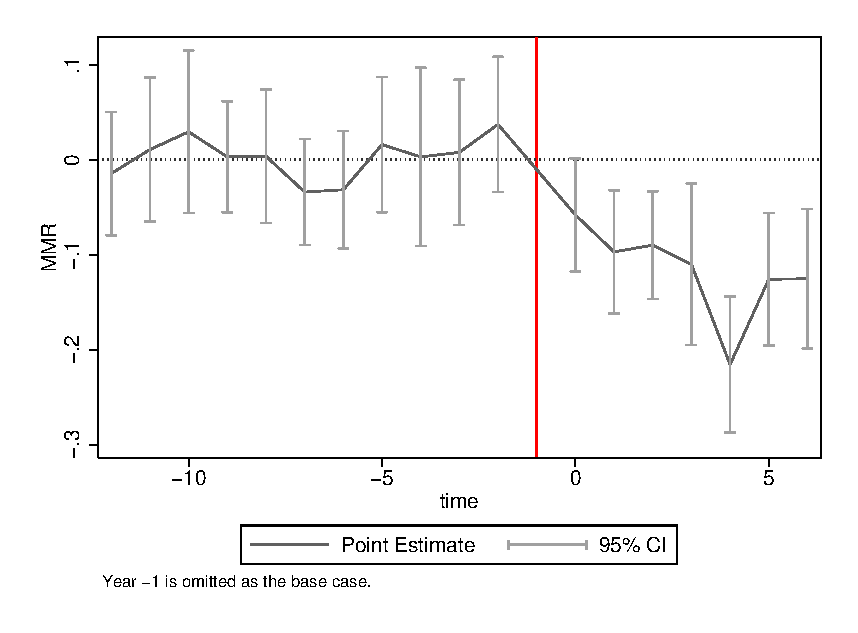
\includegraphics[scale=0.8]{./figures/eventMMR.eps}
\end{figure}
\end{frame}

\begin{frame}[IPREvent,plain]
\begin{figure}
\caption{Pneumonia (Placebo) Event Study Plot}
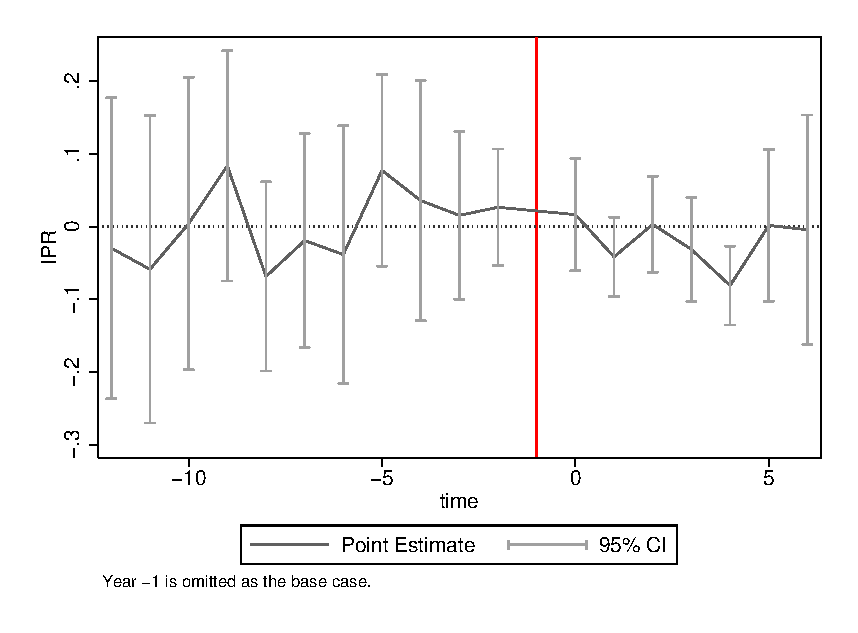
\includegraphics[scale=0.8]{./figures/eventIPR.eps}
\end{figure}
\end{frame}

%********************************************************************************
\begin{frame}[label=CC1]
\frametitle{(2) Cross-Country Evidence}
\begin{figure}[htpb!]
\centering
\begin{subfigure}{.5\textwidth}
  \centering
  \includegraphics[scale=0.39]{./figures/lLErGDP2010.eps}
  \caption{F/M Life Expectancy and GDP}
  \label{TWINfig:fertrend}
\end{subfigure}%
\begin{subfigure}{.5\textwidth}
  \centering
  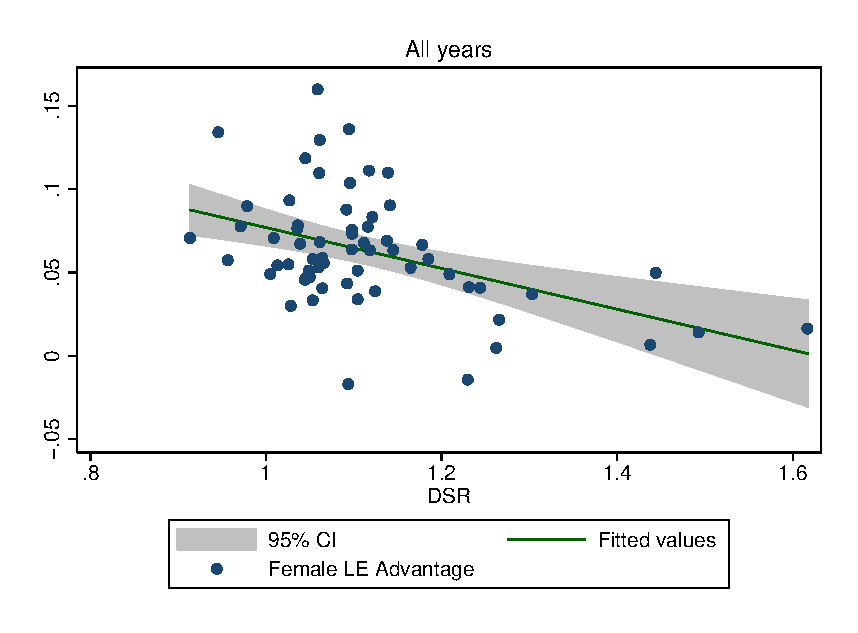
\includegraphics[scale=0.39]{./figures/lLErdesiredall.eps}
  \caption{F/M Life Exp and gender bias}
  \label{TWINfig:eductrend}
\end{subfigure}
\end{figure}
\begin{itemize}
\item Simple trends suggest \hyperlink{trends}{\textcolor{blue}{strong 
      relationship}} between LE and GDP
\item However, this is not the case for life expectancy \emph{ratio}
\item LE ratio (and \hyperlink{MMRBias}{\textcolor{blue}{MMR}}) much more 
      strongly related to gender bias
\end{itemize}
\end{frame}


\begin{frame}[label=CC]
\frametitle{Conditional Analysis}
We estimate the following regression using panel data:
	\begin{equation}
		MMR_{it} = \alpha + \beta GenderBias_{it} + \gamma_i + \delta_t + 
               (\phi_i\times t) + \theta X_{it} + \varepsilon_{it}. \nonumber
	\end{equation}
\begin{itemize}
	\item MMR is later replaced with the log ratio of female-male life expectancy.
  \item $GenderBias_{it}$ is measured as desired sex ratio of births, women's 
        rights and women's share of parliamentary seats.
	\item $\gamma$, $\delta$, $(\phi_i\times t)$ - country and year specific FE,
        country specific trends.  
  \item $X_{it}$ includes ln(GDP), interactions
	\item Standard errors are always clustered at the country level.
  \item We construct/collect \hyperlink{DSR}{\textcolor{blue}{data}} from various
        sources: WB, WHO, DHS
\end{itemize}
\end{frame}

\begin{frame}
\frametitle{Gender Bias Proxied by Desired Sex Ratio}
\begin{table}[htbp]\centering
\def\sym#1{\ifmmode^{#1}\else\(^{#1}\)\fi}
\caption{MMR and Desired Sex Ratio (boys/girls)}
\scalebox{0.7}{
\begin{tabular}{l*{5}{c}}
\toprule
                    &\multicolumn{1}{c}{(1)}   &\multicolumn{1}{c}{(2)}   &\multicolumn{1}{c}{(3)}   &\multicolumn{1}{c}{(4)}   &\multicolumn{1}{c}{(5)}   \\
                    &     MMR \ \   &     MMR \ \   &     MMR \ \   &     MMR \ \   &     MMR \ \   \\
\midrule
Desired Sex Ratio   &       824.7** &       655.0** &       667.0** &       923.9***&      2627.7***\\
                    &     [329.4]   &     [299.3]   &     [286.5]   &     [252.9]   &     [617.9]   \\
ln(GDP)             &               &               &        40.9   &        12.4   &       318.5***\\
                    &               &               &      [48.5]   &      [49.8]   &     [119.6]   \\
Desired Sex Ratio$\times$ ln(GDP)&               &               &               &               &      -285.3***\\
                    &               &               &               &               &     [100.7]   \\
Constant            &      -476.0   &      -405.1   &      -712.6   &     -1514.3***&     -3371.0***\\
                    &     [358.9]   &     [325.8]   &     [494.2]   &     [483.9]   &     [734.5]   \\
\midrule
R-squared           &        0.09   &        0.92   &        0.92   &        0.93   &        0.93   \\
Observations        &         310   &         310   &         307   &         307   &         307   \\
 Country FE &&Y&Y&Y&Y\\ Year FE&&Y&Y&Y&Y\\ 
Desired Fertility&&&&Y&Y\\
\bottomrule\end{tabular}}\end{table}

\end{frame}

\begin{frame}
\frametitle{Gender Bias Measured by Women's Rights (Cingranelli et al., 2013)}
\input{./tables/rightsMMR.tex}
\end{frame}

\frame{
\frametitle{Gender Bias and Grammatical Gender}
\begin{equation}
MMR_{it} = \beta_0 + \beta_1 GII_i + \beta_2 PercentLang_i + X_{it} + X_i  + \nu_{it} \nonumber
\end{equation}
\begin{itemize}
\setlength{\itemsep}{10pt}
  \item GII is highly pre-determined but it does not vary over time. So we
        include continent FE rather than country FE.
	\item The idea is that grammatical gender reflects gender attitudes in society
	\begin{itemize}
		\item Maternity leave policy differences (Givati \& Troiano, 2012).
		\item Female labour force and political participation (Gay et al. 2013).
	\end{itemize}
%\begin{enumerate}
%\item Sex-Based Intensity Index (sbii) 
%\item Number Gender Intensity Index (ngii)
%\item Gender Assignment Intensity Index (gaii) 
%\item Gender Pronouns Intensity Index (gpii) 
%\item gii0 = ngii + sbii + gaii + gpii
%\item gii1 = ngii + sbii + gaii
%\item gii2 = ngii + sbii + gpii
%\item gtroiano = number of cases of gender differentiated pronouns.
%\end{enumerate}
\item Example: gender differentiated personal pronouns: 
	\begin{itemize}
		\item English (``He", ``She")  
		\item Spanish (\textit{``El"}, \textit{``Ella"}; \textit{``Ellos"},
          \textit{``Ellas"};\textit{``Nosotros"}, \textit{``Nosotras"};
          \textit{``Vosotros"}, \textit{``Vosotras"})
	\end{itemize}
\end{itemize}
}

\begin{frame}[plain]
\input{./tables/MMRGII.tex}
\end{frame}


%********************************************************************************
\begin{frame}
\frametitle{(3) Sub-national Variation in Gender Bias}
Cross-country evidence above provides suggestive evidence, but concerns given
that language is fixed by country, and potential for unobservables in panel 
results
\vspace{5mm}
\begin{itemize}
  \item We use time and regional variation in MMR to examine whether historically
        more biased regions progress less towards improvements in female health
        outcomes
  \item Examine subsistence types (Michalopoulos et al., 2014), and catholic
        versus protestant missions (Nunn, 2012)
  \item We observe local (sub-national) variation in these variables, so can
        capture-specific factors
\end{itemize}
\end{frame}

\begin{frame}
\frametitle{(3) Sub-national Variation in Gender Bias}
\begin{figure}
\includegraphics[scale=0.5]{./figures/Africa_subsistence.jpg}
\caption{Subsistence Types (Murdoch 1959)}
\end{figure}
\end{frame}

\begin{frame}
\frametitle{(3) Sub-national Variation in Gender Bias}
For example, Michalopoulos et al.\ (2014):
\vspace{2mm}
\begin{equation}
\label{eqn:SubType}
MMR_{itc} = \beta_0 + \beta_1 Pastoral_i + X_{it} + X_i + \alpha_t + \alpha_c + \nu_{it},
\end{equation}
\begin{itemize}
\item We use Michalopoulos et al.'s specification to test whether areas which
      were historically pastoral, have worse female health outcomes today
\item Evidence that these were historically areas with more violence towards
      women and there is lower status of women in these societies
\item Using full sister histories from DHS, we construct regional measures
      of MMR for 306 regions from 32 countries in DHS
\end{itemize}
\end{frame}







\begin{frame}
\input{./tables/subsistence.tex}
\end{frame}





%********************************************************************************
\begin{frame}
\frametitle{(4) Gender Neutral Placebo Tests}
\begin{itemize}
\setlength{\itemsep}{10pt}
  \item Tuberculosis is a ``gender neutral'' infectious disease
  \item Frequently occurring (around 9 million cases in 2013). Incidence ranges
        from less than 10 cases per 100,000 people, to greater than 1,000 per
        100,000 (ie a range very similar to MMR)
  \item We estimate the same set of specifications with the same measures of
        gender bias, replacing MMR with TB.
\end{itemize}
\end{frame}

\begin{frame}
\input{./tables/tb-DSR.tex}
\end{frame}

\begin{frame}
\input{./tables/rightstb.tex}
\end{frame}

\begin{frame}[plain]
\begin{table}[htbp]\centering
\def\sym#1{\ifmmode^{#1}\else\(^{#1}\)\fi}
\caption{TB and Gender Intensity of Language Measures}
\scalebox{0.5}{
\begin{tabular}{l*{8}{c}}
\toprule
\textsc{Dep Var}:   &\multicolumn{1}{c}{(1)}&\multicolumn{1}{c}{(2)}&\multicolumn{1}{c}{(3)}&\multicolumn{1}{c}{(4)}&\multicolumn{1}{c}{(5)}&\multicolumn{1}{c}{(6)}&\multicolumn{1}{c}{(7)}&\multicolumn{1}{c}{(8)}\\
TB Incidence        &\multicolumn{1}{c}{NGII}&\multicolumn{1}{c}{SBII}&\multicolumn{1}{c}{GPII}&\multicolumn{1}{c}{GAII}&\multicolumn{1}{c}{GII0}&\multicolumn{1}{c}{GII1}&\multicolumn{1}{c}{GII2}&\multicolumn{1}{c}{GTroiano}\\
\midrule
\multicolumn{9}{l}{\textsc{Panel A: No Interaction}}\\
Gender Intensity Index&     -35.418*  &     -38.718   &     -70.779** &      19.500   &      -2.428   &       0.655   &     -23.346** &      -0.365   \\
                    &    [18.025]   &    [26.189]   &    [28.896]   &    [29.072]   &     [7.586]   &     [9.328]   &    [10.351]   &     [4.403]   \\
ln(GDP)             &     -40.202***&     -39.557***&     -49.045***&     -21.397** &     -21.940** &     -21.906** &     -38.367***&     -27.911***\\
                    &    [12.645]   &    [12.493]   &    [14.762]   &    [10.676]   &    [10.279]   &    [10.760]   &    [12.174]   &     [6.210]   \\
R-squared           &        0.55   &        0.55   &        0.52   &        0.58   &        0.57   &        0.57   &        0.56   &        0.55   \\
Observations        &        2619   &        2619   &        2561   &        1893   &        1812   &        1893   &        2469   &        1742   \\
\\ \multicolumn{9}{l}{\textsc{Panel B: GDP Interaction}}\\
Gender Intensity Index&    -113.987   &    -106.469   &    -212.387*  &      49.996   &      -5.372   &       2.209   &     -62.639*  &      15.251   \\
                    &    [80.285]   &    [88.634]   &   [109.688]   &   [151.564]   &    [34.552]   &    [44.033]   &    [36.067]   &    [22.170]   \\
GII $\times$ ln(GDP)&       9.411   &       8.485   &      17.487   &      -3.786   &       0.384   &      -0.204   &       5.032   &      -1.779   \\
                    &     [8.283]   &     [9.232]   &    [12.137]   &    [16.701]   &     [3.870]   &     [5.102]   &     [3.871]   &     [2.310]   \\
ln(GDP)             &     -44.724***&     -45.505***&     -54.743***&     -18.746   &     -22.978   &     -21.476   &     -46.338***&     -23.369***\\
                    &    [14.407]   &    [16.554]   &    [16.091]   &    [16.231]   &    [14.999]   &    [15.856]   &    [15.425]   &     [8.129]   \\
\midrule
R-squared           &        0.56   &        0.55   &        0.52   &        0.58   &        0.57   &        0.57   &        0.56   &        0.55   \\
Observations        &        2619   &        2619   &        2561   &        1893   &        1812   &        1893   &        2469   &        1742   \\
\bottomrule 
\end{tabular}}\end{table}

\end{frame}

%********************************************************************************
\begin{frame}
\frametitle{Discussion and Conclusions}
\begin{itemize}
	\item Preventable maternal mortality is still very high in many developing 
        countries, even after falling by almost 50\% since 1990.
	\item It exhibits substantial cross-country variation conditional on income.
	\item We show that there is a consistent relationship whereby MMR conditional 
        on income varies systematically with measures of gender prejudice.
	\item Female life expectancy advantage behaves like MMR in this regard
	\item This result is, in general, robust to alternative measures of gender 
        prejudice
	\item It is evident within countries over time and in the cross-section of
        countries, it was evident in 1930s America and is evident in today's
        poorer countries.
\end{itemize}
\end{frame}



%********************************************************************************
%********************************************************************************
%*** APPENDICES
%********************************************************************************
%********************************************************************************


\begin{frame}[plain]
\begin{center}
\textbf{Appendices}
\end{center}
\end{frame}


\begin{frame}[label=Yentl]
\frametitle{The Yentl Syndrome}
From the New England Journal of Medicine: \\
\vspace{4mm}
\textit{Yentl, the 19th-century heroine of Isaac Bashevis Singer's short story, 
had to disguise herself as a man to attend school and study the Talmud. Being 
``just like a man'' has historically been a price women have had to pay for 
equality. Being different from men has meant being second-class and less than 
equal for most of recorded time and throughout most of the world. It may therefore 
be sad, but not surprising, \hyperlink{intro}{\textcolor{red}{that women have all 
too often been treated less than equally in social relations, political endeavors, 
business, education, research, and health care.}}}\\
\end{frame}


\begin{frame}[plain,label=DDreg]
\input{./tables/mechanism.tex}
{\footnotesize \hyperlink{USA}{\textcolor{blue}{back}}}
\end{frame}


\begin{frame}[plain,label=ptrends]
\begin{figure}[h!]
\centering
\caption{Trends in ln(MMR)}
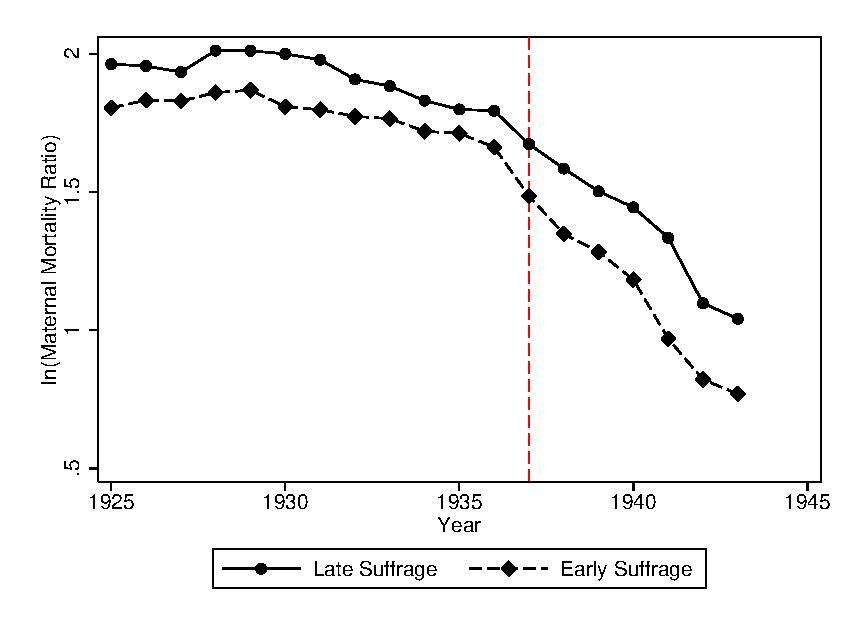
\includegraphics[scale=0.67]{./figures/MMRtrends.eps}
\end{figure}
{\footnotesize \hyperlink{USA}{\textcolor{blue}{back}}}
\end{frame}

\begin{frame}[plain,label=ptrends]
\begin{figure}[h!]
\centering
\caption{Trends in ln(IPR)}
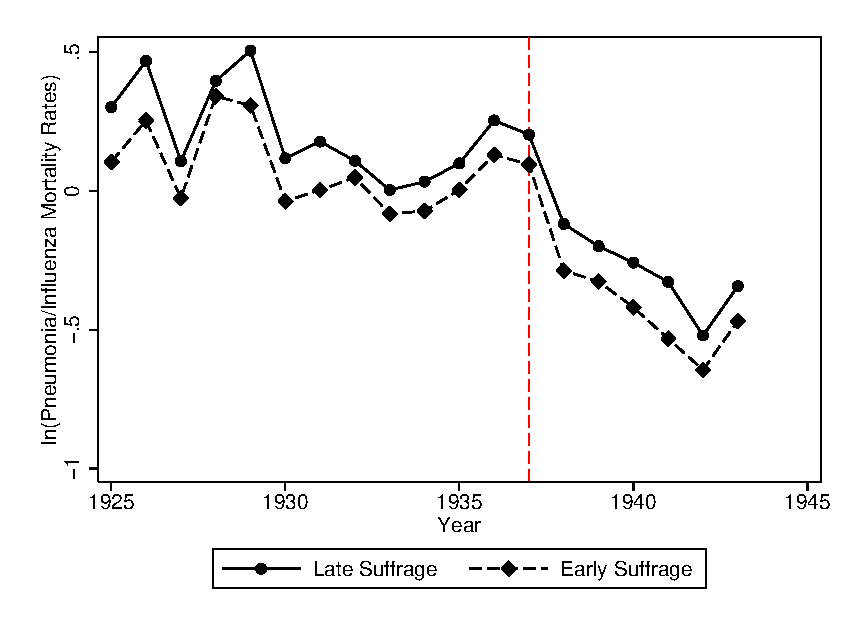
\includegraphics[scale=0.67]{./figures/IPRtrends.eps}
\end{figure}
{\footnotesize \hyperlink{USA}{\textcolor{blue}{back}}}
\end{frame}

\begin{frame}[label=DSR]
\frametitle{Gender Bias Proxied by Desired Sex Ratio}
\begin{itemize}
\item We construct time profiles of the desired sex ratio of births at the individual level using the DHS
\item The DSR in, say, 1990, is the DSR reported by all women who were 20-25 years of age in 1990, irrespective of when their responses are elicited.
\begin{itemize}
\item Low Son Preference countries: Dominican Republic (0.92); Haiti, Ukraine (0.94); Nicaragua (0.96), Colombia (0.99) 
\item Medium: Zimbabwe (1.08), Ghana (1.108), Tanzania (1.07) 
\item High: India (1.33), Nepal (1.42), Pakistan (1.59)
\end{itemize}
\item \hyperlink{DSRIMR}{\textcolor{blue}{We checked}} that DSR is strongly linked to excess girl infant mortality
\item Similar results hold when we use the life expectancy differential instead of MMR
\end{itemize}
{\footnotesize \hyperlink{CC}{\textcolor{blue}{back}}}
\end{frame}

\begin{frame}[label=trends,plain]
\begin{figure}
\caption{Female Life Expectancy and ln(GDP)}
\includegraphics[scale=0.75]{./figures/lLEGDP2010.eps}
\end{figure}
\vspace{-8mm}
{\footnotesize \hyperlink{CC1}{\textcolor{blue}{back}}}
\end{frame}

\begin{frame}[label=MMRBias,plain]
\begin{figure}
\caption{Maternal Mortality Ratio and gender bias proxy}
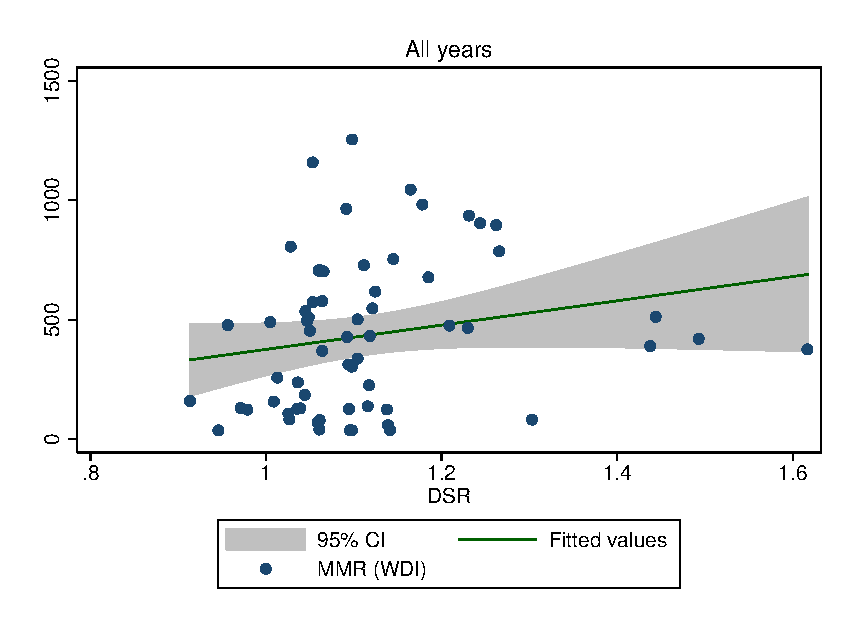
\includegraphics[scale=0.75]{./figures/lMMRWDIdesiredall.eps}
\end{figure}
\vspace{-8mm}
{\footnotesize \hyperlink{CC1}{\textcolor{blue}{back}}}
\end{frame}






\end{document}




\frame{
\frametitle{Related Literature}
\begin{itemize}
\setlength{\itemsep}{20pt}
	\item Literature on missing women
	\begin{itemize}
	\setlength{\itemsep}{10pt}
		\item Sen 1981,2003 highlights the deficit of girls age 0-5 in India.
		\item Anderson and Ray 2010, 2012 highlight missing women across the [disease and] age distribution.
		\item They are agnostic about prejudice driving excess mortality amongst women.
		\item We present the first attempt to focus on maternal mortality decline and assess the role of ``cultural factors" conditional upon income (Jayachandran 2014 discusses this in more general terms).
	\end{itemize}
\end{itemize}
}

\frame{
\frametitle{MMR: Policy initiatives are recent. Varying adoption}
\begin{itemize}
\setlength{\itemsep}{10pt}
	\item International policy initiatives directed at MMR reduction began as late as 1987 with the Safe Motherhood Initiative (Hogan et al. 2010).
	\item Enhanced commitment from the early 1990s: 1994 International Conference on Population \& Development, MMR set as an MDG.
	\item Limited progress, substantial declines only in the 2000s. 
	\item This led to the UN Secretary General launching the Every Woman Every Child Initiative and creating the Commission on Information and Accountability for Women and Children's Health in 2010 (Kassebaum et al 2014). 
\end{itemize}
}

\frame{
\frametitle{Wider Angle: Life Expectancy}
\begin{itemize}
	\item In early 20th century America, maternal mortality was the 2nd largest cause of death for women of reproductive age, after TB (which affected men equally): Alabanesi \& Olivetti (2009). 
		\begin{itemize}
	\item Similar magnitude in poor countries today although also CVD, injuries in India and HIV/AIDS in Africa.
		\end{itemize}
	\item MMR contributes to female life expectancy.
		\begin{itemize}
	\item MMR declined by around 30\% in the late 1930s in America, raising the female-male LE differential at age 20 from 1.5 years in 1920 to 6 years in 1960. 
	\item In the OECD the average female advantage in life expectancy during 1960-2011 was 6 years. 
	\item In SS-Africa it is 2-3 years and in S-Asia it is close to zero.
\end{itemize}
\end{itemize}
}

\frame{
\frametitle{Implications for Other Outcomes}
MMR decline not only contributes to improving female life expectancy and child outcomes but also other outcomes.
\begin{itemize}
\setlength{\itemsep}{14pt}
	\item MMR decline raises
		\begin{itemize}
			\item women's labour force participation (Alabanesi \& Olivetti 2009) 
			\item women's education (Alabanesi \& Olivetti (2014), Jayachandran \& Lleras-Muney 2008).
		\end{itemize}
		\item Gender equality in general and MMR decline in particular have been linked to economic growth (Lagerlof 2003, Amiri and Gerdtham 2013, Kirigia et al 2006).
		%\item MMR decline tends to raise fertility, although concurrent IMR decline tends to lower fertility (Bhalotra \& Venkataramani 2014).
\end{itemize}

}

\frame{
\frametitle{Hypothesis}
\begin{itemize}
\setlength{\itemsep}{20pt}
		\item Mechansim?
	\begin{itemize}
	\setlength{\itemsep}{15pt}
		\item Son preference - high \textit{fertility} - higher maternal mortality risk per woman (mechanical) and among higher order births (maternal depletion). e.g. Milazzo (2014).
		\begin{itemize}
			\item We investigate \textit{MMR per birth}
		\end{itemize}
		\item \textbf{Policy priorities} - resources to MMR (woman- specific) vs competing priorities: TB, infant diarrhea, pneumonia, measles, malaria. Lancet paper, Lancet editorial.
		\begin{itemize}
			\item Historical introduction of antibiotics in the US
			\item Contemporary introduction of abortion laws
			\item Reduced form approach with TB as a placebo disease
		\end{itemize}
	\end{itemize}
\end{itemize}
}



\frame{
\frametitle{Empirical Challenge: difficult to find exogenous variation in gender prejudice}
\begin{itemize}
\setlength{\itemsep}{10pt}
		\item In previous work we show that exogenous increases in women's education created by program interventions are associated with large declines in MMR (Bhalotra and Clarke 2013).
	\item Here we exploit the following variation:
		\begin{itemize}
			\item In implementation of women's suffrage across the US states in the early 20th century  (Miller 2008).
			\item In language at birth on premise that gender differentiation embedded in language structure proxies deep-set (centuries old) gender attitudes (Gay et al. 2013). 
			\item In elicited son preference in fertility
			\item In institutionalized political, economic and social rights of women. Zoom in on abortion law.
		\end{itemize}
\end{itemize}
}

\frame{
\frametitle{MMR: Brazil vs. India - A contrast}
	\begin{itemize}
	\setlength{\itemsep}{20pt}
		\item India: MMR was 390 in 100,000 and women's life expectancy advantage was 0.59 years in 2000. 
		\item Contrast with Brazil: MMR of 84 and women had a LE advantage of 6.1 years.
		\item Brazil adopted the Right to Health and implemented Universal Health Coverage and an emphasis on women's health ahead of other poor countries.
	\end{itemize}
}

%***********************DAMIAN PLEASE COULD YOU SUMMARIZE EFFECT SIZES IN TERMS OF THE DROP IN MMR IN EARLY AND LATE SUFFRAGE ADOPTERS; AND IN COUNTRIES WITH AND WITHOUT ABORTION LEGISLATION IN A NEW SLIDE THAT COMES HERE****************
%*******IF YOU THINK THE NEXT 2 SLIDES CAN EASILY BE CONDENSED GO AHEAD AND DO IT BUT IT IS NOT ESSENTIAL**(i removed desc stats slides as they were not intuitive for reader i think and too much tinkering to adjust by Tue).*

\begin{frame}
\frametitle{Overview: The Effect of Gender Equality on MMR}
Gender bias has large effects on women's health (I):
\vspace{4mm}
\begin{itemize}
	\item A 1 s.d. increase in son preference results in:
	\begin{itemize}
		\item 92 additional maternal deaths per 100,000 live births which is 21\% of the MMR mean and 27\% of the s.d. 
		\item A reduction of 24\% of the mean and 38\% of the s.d. of the relative female LE advantage. 
		\item A 62\% reduction in a girl child's survival advantage.  
	\end{itemize}
\end{itemize}
\end{frame}

\begin{frame}
\frametitle{Overview: The Effect of Gender Equality on MMR}
Gender bias has large effects on women's health (II):
\vspace{4mm}
\begin{itemize}
		\item A 1 s.d.increase in women's political rights leads to a decrease in maternal deaths of 7.11\% of the mean and 5.4\% of the s.d. 
    \item Comparing reductions in MMR in early- and late-suffrage states following the arrival of sulfanide drugs in the USA:
\begin{itemize}
		\item Early suffrage states in the USA reduced MMR by nearly 10 percentage points more than late suffrage states
    \item In comparative terms, this is approximately \emph{double} the effect seen in late-suffrage states 
\end{itemize}
\end{itemize}
\end{frame}

\begin{frame}
\frametitle{Overview: The Effect of Gender Equality on MMR}
These effects are statistically and economically significant:
\vspace{5mm}
\begin{itemize}
  \item A 1 s.d.\ reduction in gender inequality has (conditionally) the same effect on life
expectancy advantage as a 0.7 s.d.\ increase in ln(GDP)
  \item Turning to MMR, a 1 s.d.\ reduction in gender equality has slightly \emph{larger} 
effects than a 1 s.d.\ increase in ln(GDP)
  \item Country income level has similar effects on tuberculosis
  \item However gender bias has no significant effect on rates of TB
  \item Similarly, early suffrage states are no more likely than late suffrage states to employ sulfanides to reduce infant pneumonia deaths
\end{itemize}
\end{frame}



%\frame{
%\frametitle{Results Overview (MMR \& LE from WDI sample)}
%\begin{itemize}
%	%\item MMR leads to excess female mortality in reproductive ages \& lower female LE advantage.
%	\item A one s.d.increase in MMR for low income countries: 
%	\begin{itemize}
%		\item Increases excess female mortality in the reproductive ages by 35.78\% s.d. 
%		\item Reduces the female life expectancy advantage by 25.75\% s.d.
%	\end{itemize}
%	\item A 1 s.d. increase in son preference results in:
%	\begin{itemize}
%		\item 92 additional maternal deaths per 100,000 live births which is 21\% of the MMR mean and 27\% of the s.d. 
%		\item A reduction of 24\% of the mean and 38\% of the s.d. of the relative female LE advantage. 
%		\item A 62\% reduction in a girl child's survival advantage.  
%	\end{itemize}
%		\item A 1 s.d.increase in women's political rights leads to: 
%		\begin{itemize}
%			\item A decrease in maternal deaths of 7.11\% of the mean and 5.4\% of the s.d. 
%		\end{itemize}
%\end{itemize}
%}


%\frame{
%\frametitle{Results Overview (MMR \& LE from WDI sample)}
%\begin{itemize}

%	\item A 1 s.d.increase in women's economic rights leads to: 
%	\begin{itemize}
%			\item A decrease in MMR of 5.66\% of the mean and 4.37\% of the s.d.
%			\item An increase in female life expectancy advantage of 2.21\% of the mean and 4.3\% of the s.d.
%		\end{itemize}
%		\item A 1 s.d.increase in women's social rights leads to: 
%	\begin{itemize}
%			\item A decrease in MMR of 4.2\% of the mean and 3.33\% of the s.d.
%			\item An increase in female LE advantage of 3.38\% of the mean and 6.72\% of the s.d.
%	\end{itemize}
%		\item A 1 s.d.increase in (composite) gender intensity of language leads to: 
%		\begin{itemize}
%			\item An increase in MMR of 20\% of the mean and 14\% of the s.d. 
%			\item A 21\% mean and 41\% s.d. reduction in the female LE advantage.
%		\end{itemize}
%		\item No effects on cross-country TB infection rates. 
%\end{itemize}
%}


\begin{frame}[label=USA]
\frametitle{MMR and Women's Suffrage in USA}
Sulfonamide drugs caused a historic decline in MMR and IMR (Jayachandran et al.\ 2010, Bhalotra and Venktaramani 2013)
\vspace{6mm}
\begin{itemize}
\item Rapidly adopted in hospitals and outpatient settings (post-1937)
\item We ask: was the decline in MMR following introduction of the drugs a function of suffrage adoption?
\item Suffrage adoption is a proxy for progressive attitudes towards women.
\item We divide states into those that did and did not adopt suffrage prior to the national requirement in 1920 (Miller, 2008)
\item Descriptive: Trends in {\footnotesize \hyperlink{Mtrend}{\textcolor{blue}{MMR}}}, {\footnotesize \hyperlink{Ptrend}{\textcolor{blue}{IPR}}} for early [40 per cent] vs late adopters [60 per cent]
\end{itemize}
\end{frame}


\begin{frame}
\frametitle{Cross-Country Evidence}

We estimate the following regression using panel data:
	\begin{equation}
		MMR_{it} = \alpha + \beta GenderBias_{it} + \gamma_i + \delta_t + 
               (\phi_i\times t) + \theta X_{it} + \varepsilon_{it}. \nonumber
	\end{equation}
\begin{itemize}
	\item MMR is later replaced with the log ratio of female-male life expectancy.
  \item $GenderBias_{it}$ is measured as desired sex ratio of births, women's rights and women's share of parliamentary seats.
	\item $\gamma$, $\delta$, $(\phi_i\times t)$ - country and year specific FE, country specific trends.  
  \item $X_{it}$ includes ln(GDP), interactions
	\item Standard errors are always clustered at the country level.
\end{itemize}
\end{frame}

\begin{frame}[label=DSR]
\frametitle{Gender Bias Proxied by Desired Sex Ratio}
\begin{itemize}
\item We construct time profiles of the desired sex ratio of births at the individual level using the DHS
\item The DSR in, say, 1990, is the DSR reported by all women who were 20-25 years of age in 1990, irrespective of when their responses are elicited.
\begin{itemize}
\item Low Son Preference countries: Dominican Republic (0.92); Haiti, Ukraine (0.94); Nicaragua (0.96), Colombia (0.99) 
\item Medium: Zimbabwe (1.08), Ghana (1.108), Tanzania (1.07) 
\item High: India (1.33), Nepal (1.42), Pakistan (1.59)
\end{itemize}
\item \hyperlink{DSRIMR}{\textcolor{blue}{We checked}} that DSR is strongly linked to excess girl infant mortality
\item Similar results hold when we use the life expectancy differential instead of MMR
\end{itemize}
\end{frame}

\begin{frame}
\frametitle{Gender Bias Proxied by Desired Sex Ratio}
\begin{table}[htbp]\centering
\def\sym#1{\ifmmode^{#1}\else\(^{#1}\)\fi}
\caption{MMR and Desired Sex Ratio (boys/girls)}
\scalebox{0.7}{
\begin{tabular}{l*{5}{c}}
\toprule
                    &\multicolumn{1}{c}{(1)}   &\multicolumn{1}{c}{(2)}   &\multicolumn{1}{c}{(3)}   &\multicolumn{1}{c}{(4)}   &\multicolumn{1}{c}{(5)}   \\
                    &     MMR \ \   &     MMR \ \   &     MMR \ \   &     MMR \ \   &     MMR \ \   \\
\midrule
Desired Sex Ratio   &       824.7** &       655.0** &       667.0** &       923.9***&      2627.7***\\
                    &     [329.4]   &     [299.3]   &     [286.5]   &     [252.9]   &     [617.9]   \\
ln(GDP)             &               &               &        40.9   &        12.4   &       318.5***\\
                    &               &               &      [48.5]   &      [49.8]   &     [119.6]   \\
Desired Sex Ratio$\times$ ln(GDP)&               &               &               &               &      -285.3***\\
                    &               &               &               &               &     [100.7]   \\
Constant            &      -476.0   &      -405.1   &      -712.6   &     -1514.3***&     -3371.0***\\
                    &     [358.9]   &     [325.8]   &     [494.2]   &     [483.9]   &     [734.5]   \\
\midrule
R-squared           &        0.09   &        0.92   &        0.92   &        0.93   &        0.93   \\
Observations        &         310   &         310   &         307   &         307   &         307   \\
 Country FE &&Y&Y&Y&Y\\ Year FE&&Y&Y&Y&Y\\ 
Desired Fertility&&&&Y&Y\\
\bottomrule\end{tabular}}\end{table}

\end{frame}

\frame{
\frametitle{Gender Inequality II: Women's Rights}
\begin{itemize}
	\item Cingranelli et. al. 2013 data set on women's rights:
	\begin{itemize}
		%\item Political, Economic \& Social rights.
		\item Political - e.g. rights to vote, run for political office.
		\item Economic - e.g. equal pay for equal work, free choice of profession without the need to obtain a husband or male relative's consent.
		\item Social - e.g. equal inheritance, enter into marriage on a basis of equality with men.

		%rights to vote, run for political office, hold elected and appointed government positions, join political parties, petition government officials. 
		%\item Economic rights. %equal pay for equal work; free choice of profession or employment without the need to obtain a husband or male relative's consent; gainful employment without the need to obtain a husband or male relative's consent; equality in hiring and promotion practices; job security (maternity leave, unemployment benefits, no arbitrary firing or layoffs, etc...); non-discrimination by employers; be free from sexual harassment in the workplace; work at night; work in occupations classified as dangerous; work in the military and the police force.  
		%\item Social rights.  %equal inheritance; enter into marriage on a basis of equality with men; travel abroad; obtain a passport; confer citizenship to children or a husband; initiate a divorce;  own, acquire, manage, and retain property brought into marriage; participate in social, cultural, and community activities; an education; choose a residence/domicile; freedom from female genital mutilation of children and of adults without their consent; and the freedom from forced sterilization.
	\end{itemize}
\item 4 discrete values of 0, 1, 2, and 3.
\item In 2000, of the 154 countries :
	\begin{itemize}
		\item 0: 7 countries -  Afghanistan, Saudi Arabia, Kuwait and UAE. 
		\item 1: 18 countries - Pakistan, other Middle Eastern countries, Russia, Bhutan. 
		\item 2: 119 countries - Mexico, Nepal, India
		\item 3: 10 countries - Scandinavia, Canada, Germany, NZ 
		\item South Africa moved up from 1 in 1990 to 3 in 2000. 
	\end{itemize}
\end{itemize}
%{\footnotesize \hyperlink{desc}{\textcolor{blue}{back}}}
}

\frame{
\frametitle{Gender Inequality II: Women's Rights}
\begin{itemize}
	\item Democracy data from Polity IV project.
	\begin{itemize}
		\item It is discreet variable lying between 0 and 10.
		\item We use the data from 1960 -2012
		\item The MMR sample is 5 yearly from 1990 onwards
		\item The mean (sd) for democracy for the MMR sample is 5.10 (3.90)
		\item Out of the 157 countries in the data for democracy in the year 2010, 34 had the score of 10 (most democratic) and 28 had the score of 0 (least democratic)
	\end{itemize}
\end{itemize}	
}




\begin{frame}
\frametitle{Women's Rights (Cingranelli et al., 2013)}
\input{./tables/rightsMMR.tex}
\end{frame}



\begin{frame}[plain]
\begin{table}
\begin{center}
\caption{MMR and Women's Political Representation \label{MMRWPR}}
\scalebox{0.7}{
\begin{tabular}{lcccccc} \toprule 
  & MMR & MMR &MMR &MMR &MMR &MMR \\
        &\multicolumn{1}{c}{(1)}&\multicolumn{1}{c}{(2)}&\multicolumn{1}{c}{(3)}&\multicolumn{1}{c}{(4)}&\multicolumn{1}{c}{(5)}&\multicolumn{1}{c}{(6)}\\
\midrule					
Women in Parliament (\%)     &      -2.313$^{*}$  &      -3.248$^{*}$  &      -3.379$^{*}$  &      -29.69$^{***}$&      -30.46$^{***}$&      -26.79$^{***}$\\
            &     (1.358)         &     (1.766)         &     (1.961)         &     (3.971)         &     (4.067)         &     (4.234)         \\
log GDP       &      -99.10$^{***}$&      -48.24         &      -44.62         &      -87.44$^{**}$ &      -83.66$^{**}$ &      -96.79$^{**}$ \\
            &     (12.19)         &     (37.66)         &     (41.13)         &     (37.00)         &     (40.35)         &     (39.74)         \\
Democracy     &                     &                     &      -4.551         &                     &      -1.807         &      -47.50$^{***}$\\
            &                     &                     &     (4.037)         &                     &     (3.372)         &     (17.34)         \\
Rights $\times$ log GDP    &                     &                     &                     &       3.464$^{***}$&       3.597$^{***}$&       3.145$^{***}$\\
            &                     &                     &                     &     (0.463)         &     (0.490)         &     (0.504)         \\
Democracy $\times$ log GDP   &                     &                     &                     &                     &                     &       6.414$^{***}$\\
            &                     &                     &                     &                     &                     &     (2.343)         \\
%\_cons      &      1027.2\sym{***}&       654.3$^{**}$ &       665.0$^{**}$ &       939.8\sym{***}&       929.9\sym{***}&       995.4\sym{***}\\
%            &     (104.2)         &     (286.0)         &     (311.5)         &     (283.3)         &     (306.7)         &     (293.5)         \\
\midrule
N       &         659         &         659         &         594         &         659         &         594         &         594         \\
R-squared          &                     &       0.278         &       0.287         &       0.425         &       0.441         &       0.468         \\
\bottomrule
%\multicolumn{7}{p{11cm}}{\tiny The dependent variable is MMR (deaths per 100,000 live births). The regressions are based on a sample of around 158 countries for the years 1995, 2000, 2005 and 2010. All the variables are 5 yearly averages.}\\
\end{tabular}}
\end{center}
\end{table}
\end{frame}


\frame{
\frametitle{Gender Inequality III: Grammatical Gender}

\begin{equation}
MMR_{it} = \beta_0 + \beta_1 GII_i + \beta_2 PercentLang_i + X_{it} + X_i  + \nu_{it} \nonumber
\end{equation}

\begin{itemize}
\item GII is highly pre-determined but it does not vary over time. So we include continent FE rather than country FE.
\setlength{\itemsep}{10pt}
	\item The idea is that grammatical gender reflects gender attitudes in society
	\begin{itemize}
		\item Maternity leave policy differences (Givati \& Troiano, 2012).
		\item Female labour force and political participation (Gay et al. 2013).
	\end{itemize}
%\begin{enumerate}
%\item Sex-Based Intensity Index (sbii) 
%\item Number Gender Intensity Index (ngii)
%\item Gender Assignment Intensity Index (gaii) 
%\item Gender Pronouns Intensity Index (gpii) 
%\item gii0 = ngii + sbii + gaii + gpii
%\item gii1 = ngii + sbii + gaii
%\item gii2 = ngii + sbii + gpii
%\item gtroiano = number of cases of gender differentiated pronouns.
%\end{enumerate}
\item Example: gender differentiated personal pronouns: 
	\begin{itemize}
		\item English (``He", ``She")  
		\item Spanish (\textit{``El"}, \textit{``Ella"}; \textit{``Ellos"}, \textit{``Ellas"};\textit{``Nosotros"}, \textit{``Nosotras"}; \textit{``Vosotros"}, \textit{``Vosotras"})
	\end{itemize}
\end{itemize}
}

\begin{frame}[plain]
\input{./tables/MMRGII.tex}
\end{frame}

\begin{frame}
\frametitle{Placebo Tests}
\begin{itemize}
\item Tuberculosis is a ``gender neutral'' infectious disease
\item Frequently occurring (around 9 million cases in 2013). Incidence ranges from less than 10 cases per 100,000 people, to greater than 1,000 per 100,000 (ie a range very similar to MMR)
\item We estimate the same set of specifications with the same measures of gender bias, replacing MMR with TB.
\end{itemize}
\end{frame}


\begin{frame}
\input{./tables/tb-DSR.tex}
\end{frame}

\begin{frame}
\input{./tables/rightstb.tex}
\end{frame}

\begin{frame}[plain]
\begin{table}[htbp]\centering
\def\sym#1{\ifmmode^{#1}\else\(^{#1}\)\fi}
\caption{TB and Gender Intensity of Language Measures}
\scalebox{0.5}{
\begin{tabular}{l*{8}{c}}
\toprule
\textsc{Dep Var}:   &\multicolumn{1}{c}{(1)}&\multicolumn{1}{c}{(2)}&\multicolumn{1}{c}{(3)}&\multicolumn{1}{c}{(4)}&\multicolumn{1}{c}{(5)}&\multicolumn{1}{c}{(6)}&\multicolumn{1}{c}{(7)}&\multicolumn{1}{c}{(8)}\\
TB Incidence        &\multicolumn{1}{c}{NGII}&\multicolumn{1}{c}{SBII}&\multicolumn{1}{c}{GPII}&\multicolumn{1}{c}{GAII}&\multicolumn{1}{c}{GII0}&\multicolumn{1}{c}{GII1}&\multicolumn{1}{c}{GII2}&\multicolumn{1}{c}{GTroiano}\\
\midrule
\multicolumn{9}{l}{\textsc{Panel A: No Interaction}}\\
Gender Intensity Index&     -35.418*  &     -38.718   &     -70.779** &      19.500   &      -2.428   &       0.655   &     -23.346** &      -0.365   \\
                    &    [18.025]   &    [26.189]   &    [28.896]   &    [29.072]   &     [7.586]   &     [9.328]   &    [10.351]   &     [4.403]   \\
ln(GDP)             &     -40.202***&     -39.557***&     -49.045***&     -21.397** &     -21.940** &     -21.906** &     -38.367***&     -27.911***\\
                    &    [12.645]   &    [12.493]   &    [14.762]   &    [10.676]   &    [10.279]   &    [10.760]   &    [12.174]   &     [6.210]   \\
R-squared           &        0.55   &        0.55   &        0.52   &        0.58   &        0.57   &        0.57   &        0.56   &        0.55   \\
Observations        &        2619   &        2619   &        2561   &        1893   &        1812   &        1893   &        2469   &        1742   \\
\\ \multicolumn{9}{l}{\textsc{Panel B: GDP Interaction}}\\
Gender Intensity Index&    -113.987   &    -106.469   &    -212.387*  &      49.996   &      -5.372   &       2.209   &     -62.639*  &      15.251   \\
                    &    [80.285]   &    [88.634]   &   [109.688]   &   [151.564]   &    [34.552]   &    [44.033]   &    [36.067]   &    [22.170]   \\
GII $\times$ ln(GDP)&       9.411   &       8.485   &      17.487   &      -3.786   &       0.384   &      -0.204   &       5.032   &      -1.779   \\
                    &     [8.283]   &     [9.232]   &    [12.137]   &    [16.701]   &     [3.870]   &     [5.102]   &     [3.871]   &     [2.310]   \\
ln(GDP)             &     -44.724***&     -45.505***&     -54.743***&     -18.746   &     -22.978   &     -21.476   &     -46.338***&     -23.369***\\
                    &    [14.407]   &    [16.554]   &    [16.091]   &    [16.231]   &    [14.999]   &    [15.856]   &    [15.425]   &     [8.129]   \\
\midrule
R-squared           &        0.56   &        0.55   &        0.52   &        0.58   &        0.57   &        0.57   &        0.56   &        0.55   \\
Observations        &        2619   &        2619   &        2561   &        1893   &        1812   &        1893   &        2469   &        1742   \\
\bottomrule 
\end{tabular}}\end{table}

\end{frame}

\begin{frame}
\frametitle{Abortion Legislation as a Mechanism}
Gender prejudice may deter passage of abortion legislation or, conditional upon legislation, it may deter implementation.
\vspace{5mm}
\begin{itemize}
\item We coded data on abortion reforms over time for all countries 
\item Preliminary results suggest that more gender biased countries are less likely to allow abortion 
\item This is still work in progress.
\end{itemize}
\end{frame}

\begin{frame}
\input{./tables/abortionGII.tex}
\end{frame}

\begin{frame}[plain]
\begin{figure}[h!]
\centering
\caption{Introductory Analysis: Abortion Reform and MMR}
\includegraphics[scale=0.62]{./figures/eventlnMMR.eps}
\end{figure}
\vspace{-5mm}
{\footnotesize Displays difference between early and late-legislators of abortion (pre-post 1995) after the introduction of the MDGs.}
\end{frame}



\section{Conclusion}
\frame{
\frametitle{Conclusion}
\begin{itemize}

	\item Preventable maternal mortality is still very high in many developing countries, even after falling by almost 50\% since 1990.
	\item It exhibits substantial cross-country variation conditional on income.
	\item We show that there is a consistent relationship whereby MMR conditional on income varies systematically with measures of gender prejudice.
	\item Female life expectancy advantage behaves like MMR in this regard
	\item This result is, in general, robust to alternative measures of gender prejudice
	\item It is evident within countries over time and in the cross-section of countries, it was evident in 1930s America and is evident in today's poorer countries.
\end{itemize}
}




\begin{frame}[plain]
\begin{center}
{\Large Appendix Figures}
\end{center}
\end{frame}



\begin{frame}[plain,label=MMRmap]
\begin{figure}[h!]
\centering
\includegraphics[scale= 0.45]{./figures/MMR}
\caption{MMR}
\end{figure}
{\footnotesize \hyperlink{desc}{\textcolor{blue}{back}}}
\end{frame}

\begin{frame}[plain,label=LEMap]
\begin{figure}[h!]
\centering
\includegraphics[scale= 0.45]{./figures/LE_ratio}
\caption{Female Life Expectancy Advantage}
\end{figure}
{\footnotesize \hyperlink{desc}{\textcolor{blue}{back}}}
\end{frame}


\begin{frame}[plain]
\begin{center}
{\Large Appendix Tables}
\end{center}
\end{frame}


\begin{frame}[label=DSRIMR]
\frametitle{Desired Sex Ratio and Infant Mortality}
\input{./tables/DSRIMR.tex}
{\footnotesize \hyperlink{DSR}{\textcolor{blue}{back}}}
\end{frame}

\begin{frame}[label=DSRLExp]
\frametitle{Life Expectancy Differential and the Desired Sex Ratio}
\input{./tables/ln_LE_ratio-DSR.tex}
{\footnotesize \hyperlink{DSR}{\textcolor{blue}{back}}}
\end{frame}

\begin{frame}[plain,label=MMRmort]
\begin{table}[h!]\centering
\def\sym#1{\ifmmode^{#1}\else\(^{#1}\)\fi}
\caption{Gender Differences in Mortality Rates \& Maternal Mortality}
\scalebox{0.6}{
\begin{tabular}{l*{6}{c}}
\toprule
            &\multicolumn{1}{c}{(1)}&\multicolumn{1}{c}{(2)}&\multicolumn{1}{c}{(3)}&\multicolumn{1}{c}{(4)}&\multicolumn{1}{c}{(5)}&\multicolumn{1}{c}{(6)}\\
            &\multicolumn{1}{c}{(0-14)}&\multicolumn{1}{c}{(0-14)}&\multicolumn{1}{c}{(15-49)}&\multicolumn{1}{c}{(15-49)}&\multicolumn{1}{c}{(50+)}&\multicolumn{1}{c}{(50+)}\\
\hline
Low Income\\
MMR         &      -4.640         &      -10.34\sym{*}  &       16.45\sym{***}&       17.41\sym{***}&      -2.515         &      -6.470         \\
            &     (4.637)         &     (5.286)         &     (4.701)         &     (5.284)         &     (3.886)         &     (5.586)         \\
lgdp     &     -1705.0         &     -5545.6\sym{*}  &      1928.7         &      3612.3         &      -325.6         &      -124.4         \\
            &    (1698.3)         &    (2750.4)         &    (2209.5)         &    (3482.2)         &    (1421.0)         &    (2152.0)         \\
IMR ratio (F/M)&                     &     -0.0723         &                     &      -1.511         &                     &       0.777         \\
            &                     &     (0.851)         &                     &     (1.153)         &                     &     (1.188)         \\
\hline
\(N\)       &         126         &          63         &         126         &          63         &         126         &          63         \\
r2          &       0.146         &       0.374         &       0.334         &       0.408         &       0.114         &       0.218         \\
\hline\hline
Middle Income\\
MMR         &      -8.961\sym{*}  &      -12.31\sym{**} &       17.90\sym{**} &       16.08\sym{**} &      -8.991\sym{*}  &      -7.516         \\
            &     (4.751)         &     (5.769)         &     (8.767)         &     (7.762)         &     (4.971)         &     (5.191)         \\
lgdp     &      2871.7\sym{**} &      1508.4         &     -2623.8         &     -5725.8\sym{**} &      -32.36         &       801.2         \\
            &    (1261.9)         &    (2059.6)         &    (1823.4)         &    (2339.8)         &     (678.2)         &    (1003.8)         \\
IMR ratio (F/M)&                     &       0.436         &                     &       1.066         &                     &      -0.731         \\
            &                     &     (0.481)         &                     &     (0.991)         &                     &     (0.490)         \\
\hline
\(N\)       &         368         &         183         &         368         &         183         &         368         &         183         \\
R$^2$          &      0.0717         &      0.0951         &       0.108         &       0.200         &      0.0537         &       0.103         \\
\bottomrule
\end{tabular}}
\end{table}


{\footnotesize \hyperlink{DSR}{\textcolor{blue}{back}}}
\end{frame}

\begin{frame}[plain]
\begin{center}
{\Large Appendix Details}
\end{center}
\end{frame}

\begin{frame}[label=dataapp]
\frametitle{Data Appendix (1 of 3)}
\begin{itemize}
	\item The data on Life Expectancy come from the the World Bank WDI
	\begin{itemize}
		\item ``The average number of years a newborn is expected to live if mortality patterns at the time of its birth remain constant in the future." 
		\item Female LE advantage = $ln(\frac{\text{female LE}}{\text{male LE}})*100000$ (Mean - 7066.99   s.d. - 3368.102)
		\item Available yearly from 1960-2011.
		\item Converted to 5 yearly data centering on the year.
	\end{itemize}
	\item Maternal mortality ratio (MMR) also from the WDI/WHO  	
	\begin{itemize}
		\item ``The number of women who die from pregnancy-related causes while pregnant or within 42 days of pregnancy termination per 100,000 live births."
		\item Available for 5 time periods -1990, 1995, 2000, 2005, 2010.
	\end{itemize}
\end{itemize}
\end{frame}


\begin{frame}
\frametitle{Gender Inequality I: Desired Sex Ratio}
\begin{itemize}
\setlength{\itemsep}{20pt}
	\item Each surveyed woman is asked about the ideal number of children, boys, and girls she would like to have. 
	\item	$DSR \equiv \text{Desired Sex ratio} \equiv \frac{\text{ideal no. of boys}}{\text{ideal no. of girls}}$
	\item We calculate individual and cohort-country-time specific measures of DSR. 
\begin{itemize}
		\item Low Son Preference countries: Dominican Republic (0.92); Haiti, Ukraine (0.94); Nicaragua (0.96), Colombia (0.99) 
		\item Medium Son Preference countries: Zimbabwe (1.08), Ghana (1.108), Tanzania (1.07) 
		\item High Son Preference countries: India (1.33), Nepal (1.42), Pakistan (1.59)
\end{itemize}
%\item Milazzo 2014: In order to achieve desired sex composition of children families in India:
   	%\begin{itemize}
		%\item Indulge in sex selective abortion.
		%\item Son preferring fertility behaviour (repeated and closely spaced pregnancies)
	%\end{itemize}
\end{itemize}
\end{frame}





\end{document}
{\footnotesize \hyperlink{}{\textcolor{blue}{}}}
%%%%%%%%%%%%%%%%%%%%%%%%%%%%%%%%%%%%%%%%%%%%%%%%%%%%%%%%%%%%%%%%%%%%%%%%%%%%%%%%%%%%%%%%%%%%%%
%%%%%%%%%%%%%%%%%%%%%%%%%%%%%%%%%%%%%%%%%%%%%%%%%%%%%%%%%%%%%%%%%%%%%%%%%%%%%%%%%%%%%%%%%%%%%%
%%%%%%%%%%%%%%%%%%%%%%%%%%%%%%%%%%%%%%%%%%%%%%%%%%%%%%%%%%%%%%%%%%%%%%%%%%%%%%%%%%%%%%%%%%%%%%
%%%%%%%%%%%%%%%%%%%%%%%%%%%%%%%%%%%%%%%%%%%%%%%%%%%%%%%%%%%%%%%%%%%%%%%%%%%%%%%%%%%%%%%%%%%%%%
%%%%%%%%%%%%%%%%%%%%%%%%%%%%%%%%%%%%%%%%%%%%%%%%%%%%%%%%%%%%%%%%%%%%%%%%%%%%%%%%%%%%%%%%%%%%%%
%%%%%%%%%%%%%%%%%%%%%%%%%%%%%%%%%%%%%%%%%%%%%%%%%%%%%%%%%%%%%%%%%%%%%%%%%%%%%%%%%%%%%%%%%%%%%%
%%%%%%%%%%%%%%%%%%%%%%%%%%%%%%%%%%%%%%%%%%%%%%%%%%%%%%%%%%%%%%%%%%%%%%%%%%%%%%%%%%%%%%%%%%%%%%
%%%%%%%%%%%%%%%%%%%%%%%%%%%%%%%%%%%%%%%%%%%%%%%%%%%%%%%%%%%%%%%%%%%%%%%%%%%%%%%%%%%%%%%%%%%%%%
%%%%%%%%%%%%%%%%%%%%%%%%%%%%%%%%%%%%%%%%%%%%%%%%%%%%%%%%%%%%%%%%%%%%%%%%%%%%%%%%%%%%%%%%%%%%%%
%%%%%%%%%%%%%%%%%%%%%%%%%%%%%%%%%%%%%%%%%%%%%%%%%%%%%%%%%%%%%%%%%%%%%%%%%%%%%%%%%%%%%%%%%%%%%%
%%%%%%%%%%%%%%%%%%%%%%%%%%%%%%%%%%%%%%%%%%%%%%%%%%%%%%%%%%%%%%%%%%%%%%%%%%%%%%%%%%%%%%%%%%%%%%























\frame[plain]{
\begin{figure}[h!]
\centering
\includegraphics[scale= 0.2]{lLEGDP2010}
\end{figure}

\begin{figure}[h!]
\centering
\includegraphics[scale= 0.2]{lLErGDP2010}
\end{figure}
}

\frame[plain]{
\begin{figure}[h!]
\centering
\includegraphics[scale= 0.2]{lMMRWDIGDP2010}
\end{figure}
\clearpage
}


\frame[plain]{
\begin{figure}[h!]
\centering
\includegraphics[scale= 0.15]{lMMRWDIgenderall}
\end{figure}

\begin{figure}[h!]
\centering
\includegraphics[scale= 0.15]{lLErgenderall}
\end{figure}
}





\frame{
\frametitle{Roadmap}
\begin{itemize}
\setlength{\itemsep}{20pt}
	\item Contributions of MMR to excess female mortality in reproductive ages.
	\item Three different measures of Gender inequality:
	\begin{itemize}
		\item Individual level and time varying country specific measures of Desired Sex Ratio among mothers (DHS data).
		\item Women's political, economic and social rights from Cingarelli et al. (\& women's parliamentary representation from WDI).
		\item Gender intensity of language grammar (Gay et al. 2013, G \& T, 2012) . 	
	\end{itemize}
	\item The effects of each of the above on MMR.
	\item Robustness and extensions
\end{itemize}
}






\section{Empirical Analysis}

\subsection{Methodology}
\frame{
\frametitle{Methodology}
\begin{itemize}
	\item We begin by estimating the following regression using the panel data:
	\begin{equation}
		FemaleHealth_{it} = \alpha + \beta GenderBias_{it} + \gamma_i + \delta_t + 
               (\phi_i\times t) + \theta X_{it} + \varepsilon_{it}.
	\end{equation}
	\item $FemaleHealth_{it}$ is a measure outcomes speficic to women in country $i$ and time $t$.
	\item $\gamma$ - country-specific fixed effects.  
	\item $\delta$ - year specific fixed effects. 
	\item $(\phi_i\times t)$ -  differential trends in female health measures by country.  	
	\item $\varepsilon_{it}$ - Error Term.
	\item Standard errors are always clustered at the country level.
\end{itemize}
}



\subsection{Data}
\frame{
\frametitle{Data}
\begin{itemize}
	\item The data on Life Expectancy come from the the World Bank WDI
	\begin{itemize}
		\item ``The average number of years a newborn is expected to live if mortality patterns at the time of its birth remain constant in the future." 
		\item Female LE advantage = $ln(\frac{\text{female LE}}{\text{male LE}})*100000$ (Mean - 7066.99   s.d. - 3368.102)
		\item Available yearly from 1960-2011.
		\item Converted to 5 yearly data centering on the year.
	\end{itemize}
	\item Maternal mortality ratio (MMR) also from the WDI/WHO  	
	\begin{itemize}
		\item ``The number of women who die from pregnancy-related causes while pregnant or within 42 days of pregnancy termination per 100,000 live births."
		\item Available for 5 time periods -1990, 1995, 2000, 2005, 2010.
	\end{itemize}
\end{itemize}
}


%\frame{
%\frametitle{Data}
%\begin{itemize}
	%\item Mortality rates come from the UN Mortality tables. 	
	%\item Excess Female Mortality = $ln(\frac{\text{female mortality in age category X}}{\text{male mortality in age category X}})*100000$; 
		%\begin{itemize}
			%\item where X can be (0-14), (15-49), or, (50 +).  
			%\item male (female) mortality in age category X: Percentage of male (female) deaths by broad age group (per 100 male (female)  total population);
		%\end{itemize}	
%\item This data is available at a 5 yearly intervals, from the years 1955-2005
%\end{itemize}
%}
%
%
%





\section{The Importance of Gender Inequality}


\frame{
\frametitle{Gender Inequality I: Desired Sex Ratio}
\begin{itemize}
\setlength{\itemsep}{20pt}
	\item Each surveyed woman is asked about the ideal number of children, boys, and girls she would like to have. 
	\item	$DSR \equiv \text{Desired Sex ratio} \equiv \frac{\text{ideal no. of boys}}{\text{ideal no. of girls}}$
	\item We calculate individual and cohort-country-time specific measures of DSR. 
\begin{itemize}
		\item Low Son Preference countries: Dominican Republic (0.92); Haiti, Ukraine (0.94); Nicaragua (0.96), Colombia (0.99) 
		\item Medium Son Preference countries: Zimbabwe (1.08), Ghana (1.108), Tanzania (1.07) 
		\item High Son Preference countries: India (1.33), Nepal (1.42), Pakistan (1.59)
\end{itemize}
%\item Milazzo 2014: In order to achieve desired sex composition of children families in India:
   	%\begin{itemize}
		%\item Indulge in sex selective abortion.
		%\item Son preferring fertility behaviour (repeated and closely spaced pregnancies)
	%\end{itemize}
\end{itemize}
}

\frame[plain]{
\begin{figure}[h!]
\centering
\includegraphics[scale= 0.45]{DSR}
\caption{DSR}
\end{figure}
}







\frame[plain]{
\begin{table}[htbp]\centering
\def\sym#1{\ifmmode^{#1}\else\(^{#1}\)\fi}
\tiny
\caption{MMR \& DSR  (boys/girls)  \label{MMRdsr25}}
\begin{tabular}{l*{5}{c}}iline\hline
            &\multicolumn{1}{c}{(1)}&\multicolumn{1}{c}{(2)}&\multicolumn{1}{c}{(3)}&\multicolumn{1}{c}{(4)} &\multicolumn{1}{c}{(5)}\\
\hline
Desired Sex Ratio         &      1155.2\sym{**} &       655.0\sym{**} &       667.0\sym{**} &       923.9\sym{***}&      2627.7\sym{***}\\
            &     (453.3)         &     (267.0)         &     (255.2)         &     (225.1)         &    (549.9)         \\

log GDP      &                     &                     &       40.90         &       12.38         &          318.5\sym{***}\\
            &                     &                     &     (43.20)         &     (44.36)         &    (106.4)         \\

%Desired Fertility&                     &                     &                     &       217.8\sym{***}&     225.6\sym{***}\\
%            &                     &                     &                     &     (71.23)         &       (69.20)         \\

Desired Sex Ratio* lGDP      &                     &                     &                     &                     &        -285.3\sym{***}\\
            &                     &                     &                     &                     &      (89.61)         \\

%\_cons      &      -844.8$^{*}$  &      -193.6         &      -464.1         &     -1458.7\sym{***}&     -3322.4\sym{***}\\
%            &     (504.0)         &     (297.7)         &     (413.8)         &     (431.3)         &        (640.8)         \\
\hline
Desired Fertility&     No         &         No         &     No         &     Yes        &     Yes              \\
\hline
\(N\)       &         310         &         310         &         307         &         307         &           307         \\
r2          &                     &       0.442         &       0.444         &       0.505         &        0.520         \\
\hline\hline
\multicolumn{6}{p{9cm}}{\tiny The dependent variables is MMR (deaths per 100,000 births). The regressions are based on the DHS sample (developing countries) of 63 countries for the years 1990, 1995, 2000, 2005, and 2010}\\
\end{tabular}
\end{table}
}








\frame[plain]{
\begin{table}[h!]\centering
\def\sym#1{\ifmmode^{#1}\else\(^{#1}\)\fi}
\tiny
\caption{MMR and Women's Political Rights}
\begin{tabular}{l*{6}{c}}
\hline\hline
            &\multicolumn{1}{c}{(1)}&\multicolumn{1}{c}{(2)}&\multicolumn{1}{c}{(3)}&\multicolumn{1}{c}{(4)}&\multicolumn{1}{c}{(5)}&\multicolumn{1}{c}{(6)}\\
            %&\multicolumn{1}{c}{indep1}&\multicolumn{1}{c}{indep2}&\multicolumn{1}{c}{indep3}&\multicolumn{1}{c}{indep4}&\multicolumn{1}{c}{indep5}\\
\hline
Political Rights&      -17.48         &      -9.836         &      -2.467         &      -365.7\sym{***}&      -346.9\sym{***}&      -256.7\sym{***}\\
            &     (14.61)         &     (15.33)         &     (15.35)         &     (55.99)         &     (68.86)         &     (71.24)         \\
log GDP     &      -93.60\sym{***}&       1.836         &       6.242         &      -91.71\sym{***}&      -85.10\sym{***}&      -108.9\sym{***}\\
            &     (11.00)         &     (22.53)         &     (23.43)         &     (24.88)         &     (26.76)         &     (29.37)         \\
Democracy     &                     &                     &      -10.02\sym{***}&                     &      -6.489$^{*}$  &      -72.51\sym{***}\\
            &                     &                     &     (3.686)         &                     &     (3.487)         &     (14.98)         \\
Rights * log GDP   &                     &                     &                     &       47.47\sym{***}&       45.42\sym{***}&       35.17\sym{***}\\
            &                     &                     &                     &     (6.780)         &     (8.244)         &     (8.257)         \\
Democracy * log GDP   &                     &                     &                     &                     &                     &       9.658\sym{***}\\
            &                     &                     &                     &                     &                     &     (2.090)         \\
%\_cons      &      1018.8\sym{***}&       300.8$^{*}$  &       308.0$^{*}$  &       996.5\sym{***}&       976.8\sym{***}&      1071.0\sym{***}\\
%            &     (99.16)         &     (169.3)         &     (178.1)         &     (191.8)         &     (208.2)         &     (216.8)         \\
\hline
\(N\)       &         821         &         821         &         757         &         821         &         757         &         757         \\
r2          &                     &       0.233         &       0.253         &       0.314         &       0.316         &       0.368         \\
\hline\hline
\multicolumn{7}{p{10cm}}{\tiny The dependent variable is MMR (deaths per 100,000 live births). The regressions are based on a sample of around 160 countries for the years 1990, 1995, 2000, 2005 and 2010. All the variables are 5 yearly averages.}\\
\end{tabular}
\end{table}
}



%\frame[plain]{
%\begin{table}[h!]\centering
%\def\sym#1{\ifmmode^{#1}\else\(^{#1}\)\fi}
%\tiny
%\caption{MMR and Women's Economic Rights}
%\begin{tabular}{l*{6}{c}}
%\hline\hline
            %&\multicolumn{1}{c}{(1)}&\multicolumn{1}{c}{(2)}&\multicolumn{1}{c}{(3)}&\multicolumn{1}{c}{(4)}&\multicolumn{1}{c}{(5)}&\multicolumn{1}{c}{(6)}\\
            %%&\multicolumn{1}{c}{indep1}&\multicolumn{1}{c}{indep2}&\multicolumn{1}{c}{indep3}&\multicolumn{1}{c}{indep4}&\multicolumn{1}{c}{indep5}\\
%\hline
%Economic Rights&   -0.813         &       14.25         &       6.624         &      -168.2$^{*}$  &      -164.6\sym{*}  &      -103.7         \\
            %&     (15.40)         &     (18.62)         &     (19.73)         &     (85.58)         &     (86.29)         &     (77.16)         \\
%lgdp      &      -92.78\sym{***}&       4.218         &       7.289         &      -15.72         &      -11.67         &      -55.91\sym{*}  \\
            %&     (10.68)         &     (23.13)         &     (23.96)         &     (27.60)         &     (28.19)         &     (32.58)         \\
%democ     &                     &                     &      -9.718\sym{***}&                     &      -9.448\sym{**} &      -82.79\sym{***}\\
            %&                     &                     &     (3.679)         &                     &     (3.713)         &     (14.59)         \\
%Rights * lGDP   &                     &                     &                     &       22.95\sym{**} &       21.65\sym{**} &       12.72         \\
            %&                     &                     &                     &     (9.059)         &     (9.033)         &     (7.929)         \\
%Democracy * lGDP   &                     &                     &                     &                     &                     &       10.80\sym{***}\\
            %&                     &                     &                     &                     &                     &     (2.003)         \\
%%\_cons      &       984.1\sym{***}&       246.4         &       284.2         &       401.3\sym{*}  &       429.1\sym{*}  &       697.6\sym{***}\\
%%            &     (97.48)         &     (183.1)         &     (192.1)         &     (221.9)         &     (228.5)         &     (252.9)         \\
%\hline
%\(N\)       &         819         &         819         &         755         &         819         &         755         &         755         \\
%r2          &                     &       0.233         &       0.252         &       0.251         &       0.268         &       0.335         \\
%\hline\hline
%\multicolumn{7}{p{9cm}}{\tiny The dependent variable is MMR (deaths per 100,000 live births). The regressions are based on a sample of around 160 countries for the years 1990, 1995, 2000, 2005 and 2010. All the variables are 5 yearly averages.}\\
%\end{tabular}
%\end{table}
%}
%
%
%\frame[plain]{
%\begin{table}[h!]\centering
%\def\sym#1{\ifmmode^{#1}\else\(^{#1}\)\fi}
%\tiny
%\caption{MMR and Women's Social Rights}
%\begin{tabular}{l*{6}{c}}
%\hline\hline
            %&\multicolumn{1}{c}{(1)}&\multicolumn{1}{c}{(2)}&\multicolumn{1}{c}{(3)}&\multicolumn{1}{c}{(4)}&\multicolumn{1}{c}{(5)}&\multicolumn{1}{c}{(6)}\\
            %%&\multicolumn{1}{c}{indep1}&\multicolumn{1}{c}{indep2}&\multicolumn{1}{c}{indep3}&\multicolumn{1}{c}{indep4}&\multicolumn{1}{c}{indep5}\\
%\hline
%Social Rights&       0.966         &       12.33         &       11.33         &      -151.9\sym{*}  &      -150.8\sym{*}  &      -97.87         \\
            %&     (12.17)         &     (14.01)         &     (14.30)         &     (85.02)         &     (86.55)         &     (79.49)         \\
%lgdp      &      -101.7\sym{***}&       5.772         &       2.031         &      -17.63         &      -20.93         &      -74.02\sym{**} \\
            %&     (11.60)         &     (22.34)         &     (23.00)         &     (24.45)         &     (25.13)         &     (31.68)         \\
%democ     &                     &                     &      -5.841\sym{*}  &                     &      -5.759\sym{*}  &      -76.74\sym{***}\\
            %&                     &                     &     (3.374)         &                     &     (3.406)         &     (14.89)         \\
%Rights * lGDP   &                     &                     &                     &       21.16\sym{**} &       20.98\sym{**} &       13.54         \\
            %&                     &                     &                     &     (9.684)         &     (9.893)         &     (8.903)         \\
%Democracy * lGDP   &                     &                     &                     &                     &                     &       10.84\sym{***}\\
            %&                     &                     &                     &                     &                     &     (2.146)         \\
%%\_cons      &      1052.7\sym{***}&       246.2         &       308.7\sym{*}  &       417.9\sym{**} &       475.5\sym{**} &       794.4\sym{***}\\
%%            &     (99.13)         &     (164.1)         &     (168.8)         &     (186.2)         &     (191.0)         &     (229.8)         \\
%\hline
%\(N\)       &         635         &         635         &         591         &         635         &         591         &         591         \\
%r2          &                     &       0.198         &       0.205         &       0.218         &       0.224         &       0.282         \\
%\hline\hline
%\multicolumn{7}{p{9cm}}{\tiny The dependent variable is MMR (deaths per 100,000 live births). The regressions are based on a sample of around 160 countries for the years 1990, 1995, 2000, and 2005. All the variables are 5 yearly averages.}\\
%\end{tabular}
%\end{table}
%}





%\frame[plain]{
%\begin{table}[h!]\centering
%\def\sym#1{\ifmmode^{#1}\else\(^{#1}\)\fi}
%\tiny
%\caption{MMR and Women's Political Representation \label{MMRWPR}}
%\begin{tabular}{l*{6}{c}}
%\hline\hline
        %&\multicolumn{1}{c}{(1)}&\multicolumn{1}{c}{(2)}&\multicolumn{1}{c}{(3)}&\multicolumn{1}{c}{(4)}&\multicolumn{1}{c}{(5)}&\multicolumn{1}{c}{(6)}\\
%\hline						
%Women in Parliament (\%)     &      -2.313\sym{*}  &      -3.248\sym{*}  &      -3.379\sym{*}  &      -29.69\sym{***}&      -30.46\sym{***}&      -26.79\sym{***}\\
            %&     (1.358)         &     (1.766)         &     (1.961)         &     (3.971)         &     (4.067)         &     (4.234)         \\
%log GDP       &      -99.10\sym{***}&      -48.24         &      -44.62         &      -87.44\sym{**} &      -83.66\sym{**} &      -96.79\sym{**} \\
            %&     (12.19)         &     (37.66)         &     (41.13)         &     (37.00)         &     (40.35)         &     (39.74)         \\
%Democracy     &                     &                     &      -4.551         &                     &      -1.807         &      -47.50\sym{***}\\
            %&                     &                     &     (4.037)         &                     &     (3.372)         &     (17.34)         \\
%Rights * log GDP    &                     &                     &                     &       3.464\sym{***}&       3.597\sym{***}&       3.145\sym{***}\\
            %&                     &                     &                     &     (0.463)         &     (0.490)         &     (0.504)         \\
%Democracy * log GDP   &                     &                     &                     &                     &                     &       6.414\sym{***}\\
            %&                     &                     &                     &                     &                     &     (2.343)         \\
%%\_cons      &      1027.2\sym{***}&       654.3\sym{**} &       665.0\sym{**} &       939.8\sym{***}&       929.9\sym{***}&       995.4\sym{***}\\
%%            &     (104.2)         &     (286.0)         &     (311.5)         &     (283.3)         &     (306.7)         &     (293.5)         \\
%\hline
%\(N\)       &         659         &         659         &         594         &         659         &         594         &         594         \\
%r2          &                     &       0.278         &       0.287         &       0.425         &       0.441         &       0.468         \\
%\hline\hline
%\multicolumn{7}{p{10cm}}{\tiny The dependent variable is MMR (deaths per 100,000 live births). The regressions are based on a sample of around 158 countries for the years 1995, 2000, 2005 and 2010. All the variables are 5 yearly averages.}\\
%\end{tabular}
%\end{table}
%}








\frame{
\begin{table}[h!]\centering
\def\sym#1{\ifmmode^{#1}\else\(^{#1}\)\fi}
\tiny
\caption{Gender Intensity of Language \& Maternal Mortality}
\begin{tabular}{l*{8}{c}}
\hline\hline
            &\multicolumn{1}{c}{(1)}&\multicolumn{1}{c}{(2)}&\multicolumn{1}{c}{(3)}&\multicolumn{1}{c}{(4)}&\multicolumn{1}{c}{(5)}&\multicolumn{1}{c}{(6)}&\multicolumn{1}{c}{(7)}&\multicolumn{1}{c}{(8)}\\
            &\multicolumn{1}{c}{ngii}&\multicolumn{1}{c}{sbii}&\multicolumn{1}{c}{gaii}&\multicolumn{1}{c}{gpii}&\multicolumn{1}{c}{gii0}&\multicolumn{1}{c}{gii1}&\multicolumn{1}{c}{gii2}&\multicolumn{1}{c}{gtroiano}\\
\hline
GII         &       50.03\sym{**} &       68.52\sym{**} &       105.0\sym{***}&       56.60\sym{*}  &       30.24\sym{***}&       40.23\sym{***}&       24.90\sym{*}  &       2.832         \\
            &     (21.61)         &     (33.75)         &     (29.02)         &     (32.01)         &     (10.24)         &     (12.19)         &     (12.57)         &     (8.682)         \\
lgdp      &      -71.53\sym{***}&      -72.58\sym{***}&      -77.63\sym{***}&      -66.64\sym{***}&      -71.86\sym{***}&      -74.53\sym{***}&      -68.26\sym{***}&      -69.24\sym{***}\\
            &     (19.65)         &     (19.68)         &     (22.86)         &     (19.01)         &     (22.32)         &     (22.31)         &     (19.06)         &     (19.97)         \\
\hline
\(N\)       &         575         &         575         &         417         &         562         &         399         &         417         &         542         &         384         \\
r2          &       0.701         &       0.702         &       0.766         &       0.704         &       0.750         &       0.762         &       0.690         &       0.611         \\
\hline\hline
GII         &       368.1\sym{**} &       162.9         &       665.0\sym{***}&       499.7\sym{***}&       213.0\sym{***}&       249.4\sym{***}&       149.6\sym{*}  &       148.2\sym{*}  \\
            &     (154.7)         &     (203.8)         &     (109.2)         &     (176.4)         &     (42.13)         &     (57.73)         &     (83.73)         &     (85.26)         \\
GII\_gdp     &      -38.32\sym{**} &      -11.88         &      -69.92\sym{***}&      -55.01\sym{***}&      -23.91\sym{***}&      -27.63\sym{***}&      -16.04         &      -16.70\sym{*}  \\
            &     (17.13)         &     (23.26)         &     (12.73)         &     (20.08)         &     (5.045)         &     (6.965)         &     (9.952)         &     (9.214)         \\
lgdp      &      -52.19\sym{**} &      -64.07\sym{**} &      -27.11         &      -47.69\sym{**} &      -4.747         &      -14.31         &      -42.03         &      -25.53         \\
            &     (22.84)         &     (30.76)         &     (21.57)         &     (20.28)         &     (21.37)         &     (21.37)         &     (28.60)         &     (19.44)         \\
\hline
\(N\)       &         575         &         575         &         417         &         562         &         399         &         417         &         542         &         384         \\
r2          &       0.712         &       0.703         &       0.794         &       0.718         &       0.777         &       0.784         &       0.699         &       0.636         \\
\hline\hline
\multicolumn{9}{p{12cm}}{\tiny The dependent variables is MMR (per 100,000 live births). In Panel 1 we control the percentage of
the population speaking the majority language (for which the GII has been calculated), decade dummies, continent dummies, the log of GDP, the log of population, dummies for the World Bank Income groups classification, the percentage of population that is Protestant, Catholic and Muslim, and the proportion of the country that is tropical or subtropical. In Panel 2, we add the interaction term of log of GDP and GII in addition to the previous controls. These regressions are based on a sample of around 80 countries (column 5) and the years 1990, 1995, 2000, 2005 and 2010.}\\
\end{tabular}
\end{table}
}

\section{Placebo Tests with TB infection rates}



\frame[plain]{
\begin{table}[h!]\centering
\def\sym#1{\ifmmode^{#1}\else\(^{#1}\)\fi}
\tiny
\caption{Desired Sex ratio and TB}
\begin{tabular}{l*{6}{c}}
\hline\hline
            &\multicolumn{1}{c}{(1)}&\multicolumn{1}{c}{(2)}&\multicolumn{1}{c}{(3)}&\multicolumn{1}{c}{(4)}&\multicolumn{1}{c}{(5)}&\multicolumn{1}{c}{(6)}\\
            %&\multicolumn{1}{c}{indep1}&\multicolumn{1}{c}{indep2}&\multicolumn{1}{c}{indep3}&\multicolumn{1}{c}{indep3b}&\multicolumn{1}{c}{indep4}&\multicolumn{1}{c}{indep5}\\
\hline
Desired Sex Ratio&      -48.12         &      -98.36         &      -140.7         &      -131.9         &      -804.1         &      -794.3\sym{*}  \\
            &     (194.5)         &     (263.4)         &     (266.4)         &     (294.7)         &     (519.0)         &     (467.5)         \\

ln GDP        &                     &                     &      -54.46\sym{*}  &      -55.22         &      -174.5\sym{**} &      -173.9\sym{**} \\
            &                     &                     &     (31.75)         &     (33.66)         &     (86.96)         &     (79.76)         \\

Desired Fertility&                     &                     &                     &       8.259         &                     &       4.040         \\
            &                     &                     &                     &     (90.02)         &                     &     (89.41)         \\

Desired Sex Ratio * lGDP     &                     &                     &                     &                     &       110.6         &       109.7         \\
            &                     &                     &                     &                     &     (75.55)         &     (65.91)         \\


%\_cons      &       307.1         &       324.2         &       710.4\sym{*}  &       671.6         &      1432.5\sym{**} &      1407.6\sym{**} \\
%            &     (228.9)         &     (296.8)         &     (369.5)         &     (576.6)         &     (602.9)         &     (612.3)         \\
\hline
\(N\)       &        1407         &        1407         &        1393         &        1393         &        1393         &        1393         \\
r2          &                     &      0.0438         &      0.0625         &      0.0626         &      0.0661         &      0.0662         \\
\hline\hline
\multicolumn{7}{p{9.5cm}}{\tiny The dependent variables is TB infection rates (percent of the population). These regressions are based on a sample of 63 countries DHS countries for the years 1990-2012. This is annual data.}\\
\end{tabular}
\end{table}
}




\frame[plain]{
\begin{table}[h!]\centering
\def\sym#1{\ifmmode^{#1}\else\(^{#1}\)\fi}
\tiny
\caption{Women's Political Rights and TB }
\begin{tabular}{l*{6}{c}}
\hline\hline
            &\multicolumn{1}{c}{(1)}&\multicolumn{1}{c}{(2)}&\multicolumn{1}{c}{(3)}&\multicolumn{1}{c}{(4)}&\multicolumn{1}{c}{(5)}&\multicolumn{1}{c}{(6)}\\
\hline
Political Rights&       2.323         &       2.693         &       0.604         &      -24.02         &      -29.22         &      -29.48         \\
            &     (8.302)         &     (8.396)         &     (8.878)         &     (42.99)         &     (49.47)         &     (48.40)         \\

ln GDP        &      -46.09\sym{***}&      -37.97\sym{**} &      -39.99\sym{**} &      -44.60\sym{**} &      -47.48\sym{**} &      -47.30\sym{**} \\
            &     (10.67)         &     (16.69)         &     (17.79)         &     (17.98)         &     (18.95)         &     (22.45)         \\

Democracy &                     &                     &       3.066         &                     &       3.253         &       3.611         \\
            &                     &                     &     (2.970)         &                     &     (2.971)         &     (12.42)         \\

Right*lGDP   &                     &                     &                     &       3.494         &       3.932         &       3.961         \\
            &                     &                     &                     &     (5.130)         &     (5.837)         &     (5.662)         \\

Democracy*lGDP   &                     &                     &                     &                     &                     &     -0.0528         \\
            &                     &                     &                     &                     &                     &     (1.703)         \\
\hline
\(N\)       &        3555         &        3555         &        3163         &        3555         &        3163         &        3163         \\
r2          &                     &      0.0357         &      0.0396         &      0.0367         &      0.0406         &      0.0406         \\
\hline\hline
\multicolumn{7}{p{9.5cm}}{\tiny The dependent variables is TB infection rates (percent of the population). These regressions are based on a sample of 159 countries from across the world for the years 1990-2011. This is annual data.}\\

\end{tabular}
\end{table}
}


\frame[plain]{
\begin{table}[h!]\centering
\def\sym#1{\ifmmode^{#1}\else\(^{#1}\)\fi}
\tiny
\caption{Gender Intensity of Language and TB}
\begin{tabular}{l*{8}{c}}
\hline\hline            %&\multicolumn{1}{c}{(1)}&\multicolumn{1}{c}{(2)}&\multicolumn{1}{c}{(3)}&\multicolumn{1}{c}{(4)}&\multicolumn{1}{c}{(5)}&\multicolumn{1}{c}{(6)}&\multicolumn{1}{c}{(7)}&\multicolumn{1}{c}{(8)}\\
            &\multicolumn{1}{c}{ngii}&\multicolumn{1}{c}{sbii}&\multicolumn{1}{c}{gaii}&\multicolumn{1}{c}{gpii}&\multicolumn{1}{c}{gtroiano}&\multicolumn{1}{c}{gii0}&\multicolumn{1}{c}{gii1}&\multicolumn{1}{c}{gii2}\\
\hline\hline
GII         &      -35.19\sym{*}  &      -38.72         &       18.86         &      -70.99\sym{**} &      -2.300         &       0.718         &      -23.23\sym{**} &      -0.253         \\
            &     (18.16)         &     (26.41)         &     (28.92)         &     (29.27)         &     (7.580)         &     (9.335)         &     (10.45)         &     (4.404)         \\

lgdp        &      -40.50\sym{***}&      -39.88\sym{***}&      -21.57\sym{**} &      -49.50\sym{***}&      -22.18\sym{**} &      -22.01\sym{**} &      -38.70\sym{***}&      -27.63\sym{***}\\
            &     (12.75)         &     (12.58)         &     (10.48)         &     (14.85)         &     (10.06)         &     (10.58)         &     (12.23)         &     (6.095)         \\
\hline
\(N\)       &        2513         &        2513         &        1818         &        2458         &        1741         &        1818         &        2370         &        1674         \\
r2          &       0.558         &       0.556         &       0.582         &       0.520         &       0.579         &       0.580         &       0.563         &       0.546         \\
\hline\hline
GII         &      -115.2         &      -108.2         &       52.91         &      -216.3\sym{*}  &      -5.287         &       2.361         &      -63.16\sym{*}  &       14.97         \\
            &     (81.19)         &     (89.88)         &     (151.6)         &     (111.0)         &     (34.80)         &     (44.29)         &     (36.44)         &     (22.44)         \\

GII\_gdp     &       9.611         &       8.742         &      -4.241         &       17.99         &       0.391         &      -0.217         &       5.131         &      -1.739         \\
            &     (8.381)         &     (9.346)         &     (16.72)         &     (12.30)         &     (3.908)         &     (5.139)         &     (3.911)         &     (2.345)         \\

lgdp        &      -45.16\sym{***}&      -46.03\sym{***}&      -18.58         &      -55.44\sym{***}&      -23.25         &      -21.55         &      -46.89\sym{***}&      -23.16\sym{***}\\
            &     (14.58)         &     (16.76)         &     (16.22)         &     (16.24)         &     (15.03)         &     (15.92)         &     (15.59)         &     (8.154)         \\
\hline
\(N\)       &        2513         &        2513         &        1818         &        2458         &        1741         &        1818         &        2370         &        1674         \\
r2          &       0.560         &       0.558         &       0.582         &       0.524         &       0.579         &       0.580         &       0.566         &       0.548         \\
\hline\hline
\multicolumn{9}{p{11.5cm}}{\tiny The dependent variables is TB infection rates (percent of the population). These regressions are based on a sample of 80 countries from across the world (column 5) for the years 1990-2011. This is annual data.}\\
\end{tabular}
\end{table}
}

\section{Testing Mechanisms}
\frame{
\frametitle{US Case Study:}
\begin{itemize}
\item Exploit arrival of sulfa drugs to the US in 1937.
\item Early female suffrage states (pre-1920) more likely to adopt medical technologies to directly reduce MMR? 
%\item Early suffrage states passed suffrage laws prior to the mandated national reform in 1920.  
\begin{itemize}
	\item Estimate the following DiD (Jayachandran et al.\ (2010)):
\scriptsize
\begin{eqnarray}
log(MMR)_{st} & = \alpha + \beta \mathds{1}[Post1937]_t + \gamma(EarlySuf_{s}\times t)
                + \delta_1 (EarlySuf\times Post1937_t) \nonumber \\
              & + \delta_2 (EarlySuf\times Post1937_t\times t) + \phi_t + \mu_s
                + \upsilon_{st}.
\end{eqnarray}
\normalsize
\end{itemize}
\item Split the quantitatively important (exogenous) reduction in maternal deaths which occurred with the arrival of the first 
antibiotics into three components.  
\begin{itemize}
\item $\beta$, identifies the immediate general effect of sulfa drugs on MMR, 
\item $\delta_1$ \& $\delta_2$ test whether there are larger level and trend breaks in early suffrage states.
\end{itemize}
\item Sulfa drugs were also important in reducing morbidity and mortality from  pneumonia.  
\end{itemize}
}


\frame[plain]{
\begin{table}[h!]\centering
\def\sym#1{\ifmmode^{#1}\else\(^{#1}\)\fi}
\tiny
\caption{MMR, Pneumonia Regressions}
\begin{tabular}{l*{2}{c}}
\hline\hline
            &\multicolumn{1}{c}{(1)}&\multicolumn{1}{c}{(2)}\\
            &\multicolumn{1}{c}{Ln(MMR)}&\multicolumn{1}{c}{Ln(Pneum)}\\
\hline
           &            &            \\

      Post & -0.0917*** &     0.0087 \\

           &    -0.0298 &    -0.0215 \\

 Post*Year & -0.0891*** & -0.0611*** \\

           &    -0.0049 &    -0.0108 \\

      Year & -0.0230*** & -0.0293*** \\

           &   -0.00246 &   -0.00647 \\

{\bf Early Suffrage*Post} & {\bf -0.0849**} & {\bf -0.0459} \\

           & {\bf -0.0365} & {\bf -0.0279} \\

{\bf Early Suffrage*Post*Year} & {\bf -0.0146**} & {\bf -0.00674} \\

           & {\bf -0.00642} & {\bf -0.0128} \\

Early Suffrage*Year &      0.001 &     0.0047 \\

           &   -0.00335 &    -0.0076 \\

  Constant &   1.689*** & -0.0461*** \\

           &     -0.012 &    -0.0148 \\

           &            &            \\
\hline
Observations &        868 &        868 \\

 R-squared &      0.951 &       0.78 \\
\hline
\end{tabular}
\end{table}
 }

\frame[plain]{
\vspace{-0.6cm}
\begin{center}
\begin{figure}[htbp] \centering
%\caption{Event Study - MMR in the US}$
\hspace*{-0.23in}$%
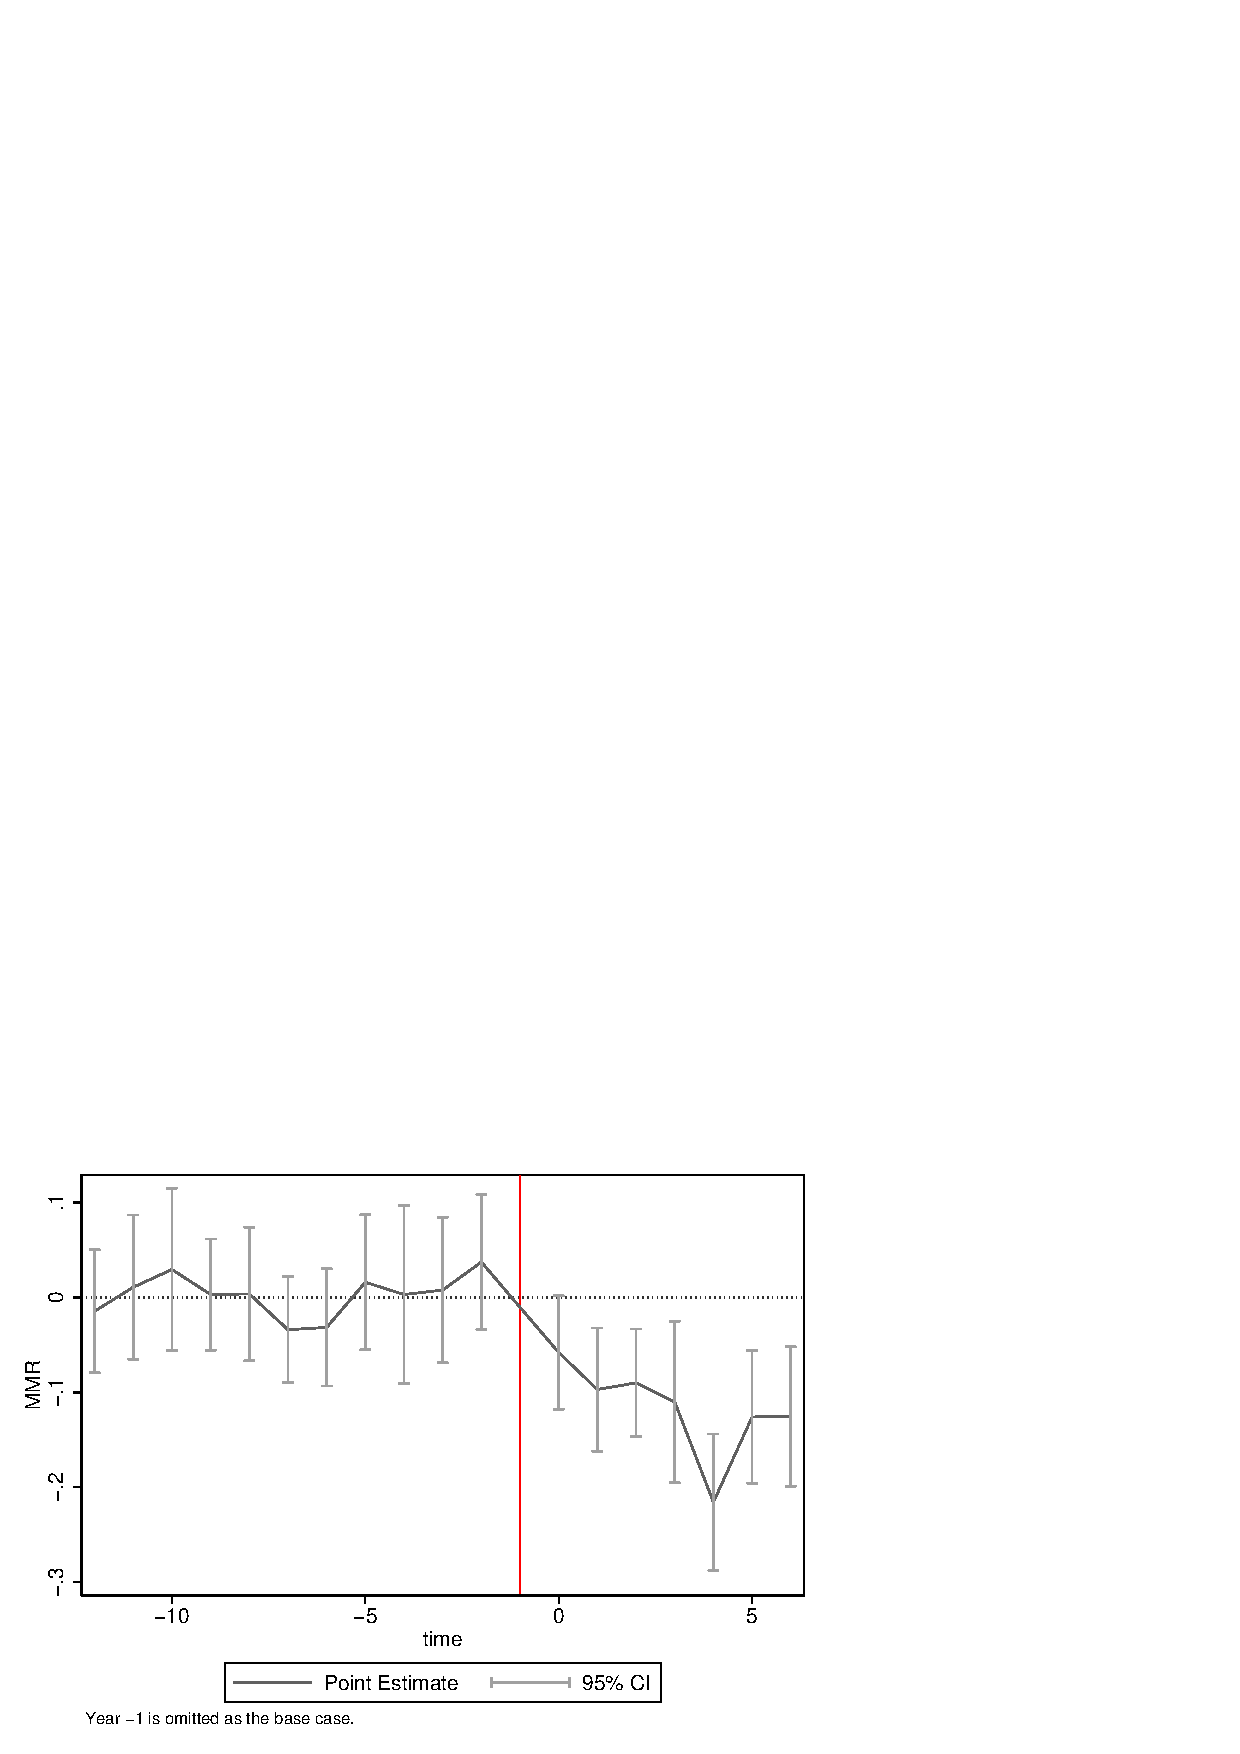
\includegraphics[scale = 0.45, trim = 7mm 0mm 0mm -3mm, clip]{./eventMMR.pdf}%
\label{Figure 2}
\end{figure}
\end{center}
\vspace{-0.9cm}
\begin{center}
\begin{figure}[htbp] \centering
%\caption{Event Study - Pneumonia in the US}$
\hspace*{-0.23in}$%
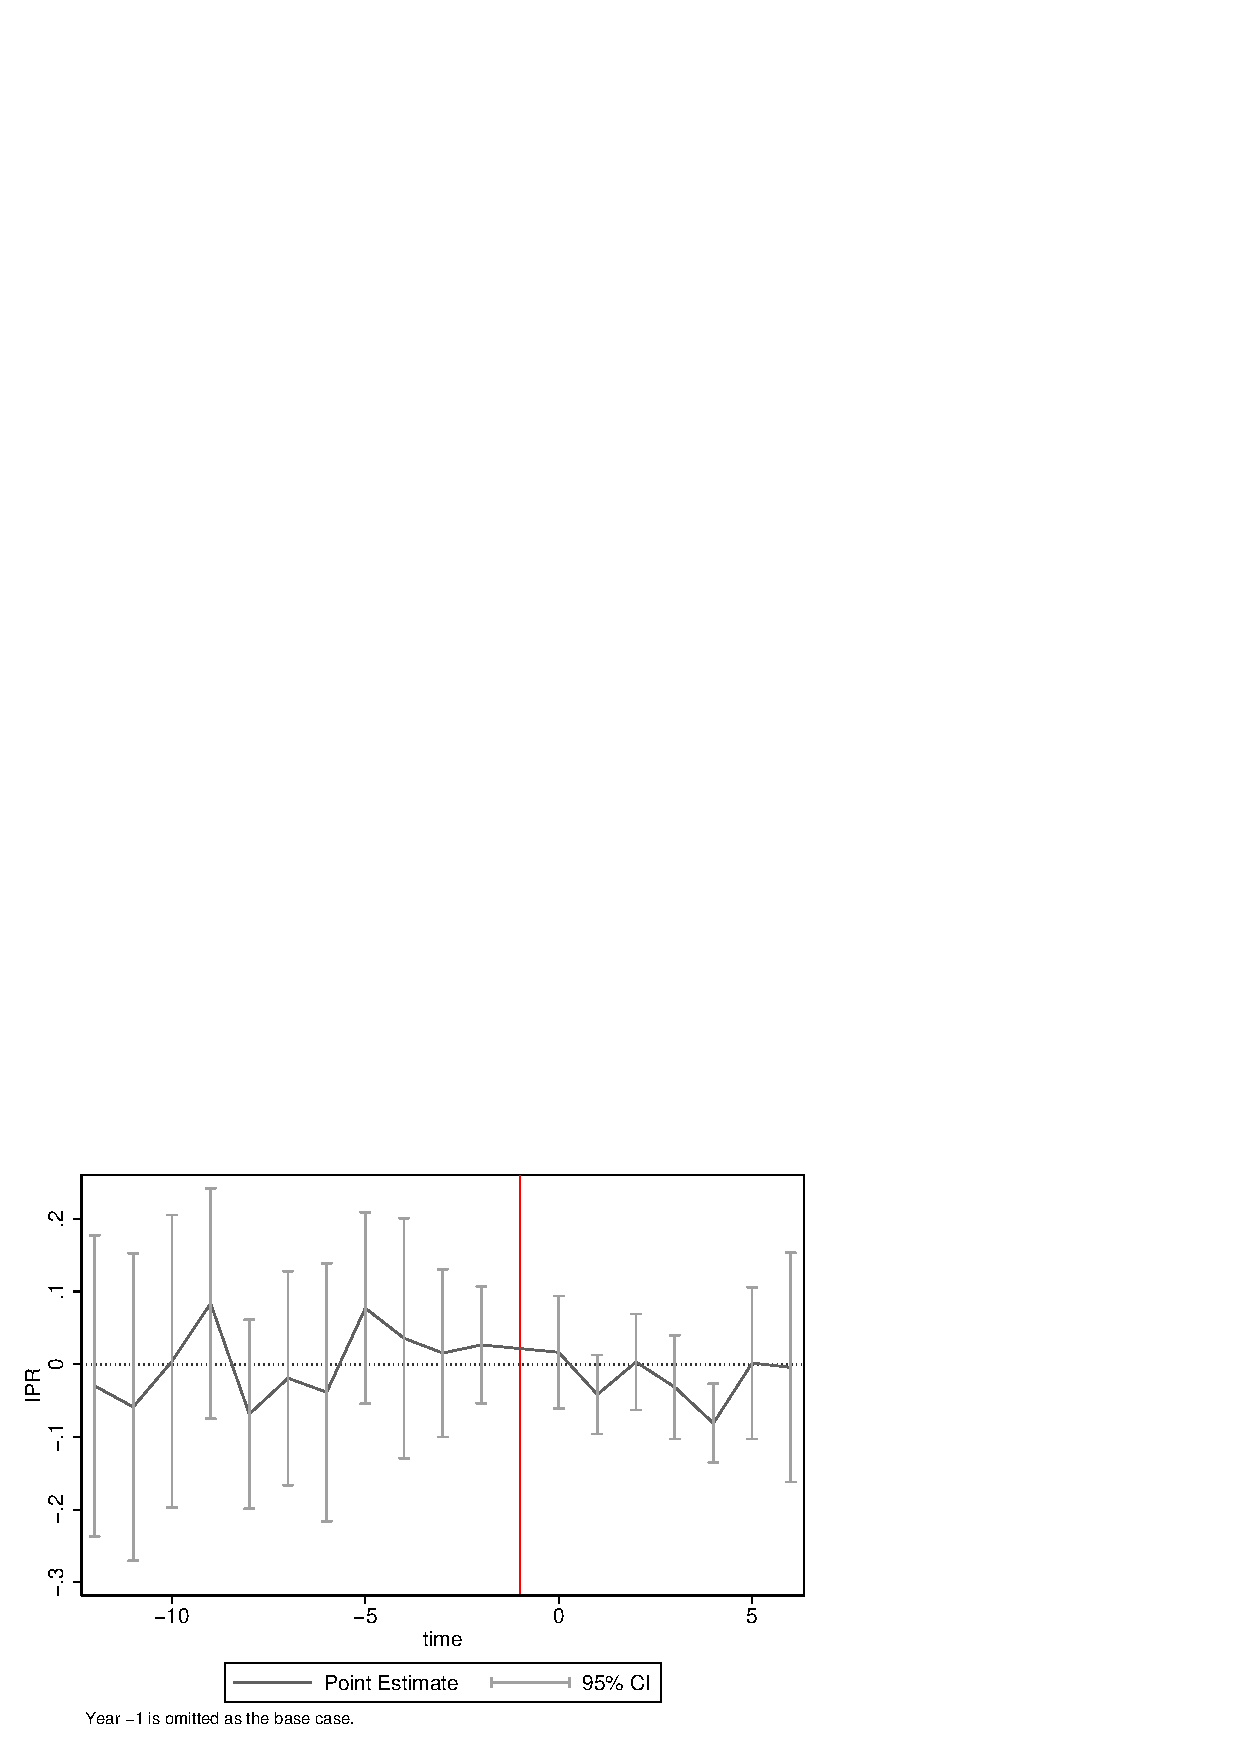
\includegraphics[scale = 0.45, trim = 7mm 0mm 0mm -3mm, clip]{./eventIPR.pdf}%
\label{Figure 3}
\end{figure}
\end{center}
}

\frame{
\frametitle{Robustness and Extensions}
\begin{itemize}
\setlength{\itemsep}{20pt}
	\item Placebo tests with TB infection rates.
	%\item While TB infection rates are gender neutral, access to treatment might not be.
	\item We replace MMR with female life expectancy advantage.
	\item Extend our country fixed effects framework to Time Varying Group Fixed Effects Framework (Bonhomme \& Manresa 2012).
	%\item Show robustness to different data sources since MMR and LE are prone to measurement difficulties.
	%\item Control for desired fertility (Jayachandran, 2014).
\end{itemize}
}

\section{Conclusion}
\frame{
\frametitle{Conclusion}
\begin{itemize}
\setlength{\itemsep}{20pt}
	\item Preventable maternal mortality is still very high in many developing countries, even after falling by almost 50\% since 1990.
	\item Substantial cross-country variation conditional on income.
	\item We show consistent relationship between MMR (and female LE advantage) and different measures of gender prejudice.
\end{itemize}
}

\renewcommand{\thetable}{\arabic{table}a}

\frame{
\begin{table}[htpb!] 
 \begin{center} 
\caption{Descriptive Statistics for Country$\times$Year Analysis}
 \label{TAB:sumstats} 
\scalebox{0.7}{
\begin{tabular}{lccccc} 
 \toprule\toprule \vspace{5mm} 
& N & Mean & Std. Dev. & Min. & Max. \\ \midrule 
\multicolumn{6}{l}{\textbf{Panel A: Health Measures}} \\ 
MMR (Deaths per 100,000 live births)&         905&      238.46&      315.79&           2&        1900\\
MMR calculated from DHS microdata&         354&      493.89&      563.90&           0&        6149\\
Life Expectancy (Male)&       10054&       60.69&       10.92&          16&          88\\
Life Expectancy (Female)&       10054&       65.27&       12.23&          23&          87\\
ln(Life Expectancy Ratio)$\times$100,000 (F/M)&       10054&     7111.35&     3454.01&       -6234&       32131\\
ln(GDP)             &        8368&        7.44&        1.68&           4&          12\\
Tuberculosis Incidence per 100,000 people&        4680&      140.28&      187.91&           0&        1826\\
 
 \bottomrule 
 \end{tabular}}\end{center}\end{table}

}
\addtocounter{table}{-1}
  \renewcommand{\thetable}{\arabic{table}b}

\begin{frame}[label=desc]
\input{./tables/sumStatsB.tex}
\vspace{4mm}
{\footnotesize
Geographic descriptives: \hyperlink{MMRmap}{\textcolor{blue}{MMR}}, \hyperlink{LEmap}{\textcolor{blue}{LE Advantage}} \\
Further definitions: \hyperlink{dataApp}{\textcolor{blue}{Data Appendix}}}
\end{frame}
\renewcommand{\thetable}{\arabic{table}}

\end{document} 

